\chapter{Linear Image Filtering}
\label{chapter:linear_image_filtering}

\section{Introduction}

We want to build a vision system that operates in the real
world.  One such system is the human visual system.  Although much remains to be understood about how
our visual system processes images, we have a fairly good idea of what happens at the initial stages of
visual processing, and it will turn out to be similar to some of the
filtering we discuss in this chapter.  While we're inspired by the
biology, here we describe some mathematically simple processing  that will
help us to parse an image into useful tokens, or {\bf low-level features} that
will be useful later to construct visual interpretations.

We'd like for our processing to enhance image structures of
use for subsequent interpretation, and to remove variability within
the image that makes more difficult comparisons with previously
learned visual signals.  Let's proceed by invoking the simplest mathematical
processing we can think of: a linear filter. Linear filters as computing structures for vision have received a lot of attention because of their surprising success in modeling some aspect of the processing carried our by early visual areas such as the retina, the lateral geniculate nucleus (LGN) and primary visual cortex (V1) \cite{Hubel62}. In this chapter we will see how far it takes us toward these goals.


For a deeper understanding there are many books~\cite{Oppenheim1996} devoted to {\bf signal processing},
\index{Signal processing}
providing essential tools for any computer vision scientist. In this chapter we will present signal processing tools from a computer vision and image processing perspective.

%\marginnote{Linear filters as computing structures for vision have received a lot of attention because of their surprising success in modeling some aspect of the processing carried our by early visual areas such as the retina, the lateral geniculate nucleus (LGN) and primary visual cortex (V1).}[-1.27cm]


%\section{Linear Filtering}

%Linear filters as computing structures for vision have received a lot of attention because of their surprising success in modeling some aspect of the processing carried our by early visual areas such as the retina, the lateral geniculate nucleus (LGN) and primary visual cortex (V1). Neurons are modeled by a linear first stage that takes a weighted linear combination of the input image and a second stage which performs a non-linearity. This model is certainly a simplification but it is remarkably successful at explaining a large number of observations in the primate visual system. 

%Many of the filters that we will review in this chapter and the next one have become popular because of their functionality as image processing tools and/or because of their fit to observations in the early visual system.



\section{Signals and Images}

A {\bf signal} is a measurement of some physical quantity (light, sound, height, temperature, etc.) as a function of another independent quantity (time, space, wavelength, etc.). A {\bf system} is a process/function that transforms a signal into another.

%In this chapter we will introduce some basic tools to characterize images and simple image processing systems. We will describe tools from signal and image processing. 

%Our goal will be to extract from images information useful to build meaningful representations of the image in order to understand its content. 

%The tools we will review here allow representing signals (1D sequences, images or movies) and the filters used to process them.

%\section{Signals, images and sequences}

\subsection{Continuous and Discrete Signals}


Although most of the signals that exist in nature are infinite {\bf continuous signals},
\index{Signals!Continuous}
when we introduce them into a computer they are sampled and transformed into a finite sequence of numbers, also called a {\bf discrete signal}.
\index{Signals!Discrete}

\marginnote{{\bf Sampling}
	\index{Signals!Sampling}
	is the process of transforming a continuous signal into a discrete one and will be studied in detail in \chap{\ref{chapter:sampling}}.}

If we consider the light that reaches one camera photo sensor, we could write it as a one dimensional function of time, $\img (t)$, where $\img (t)$ denotes the incident $\img$ight at time $t$, and $t$ is a continuous variable that can take on any real value.
The signal $\img (t)$ is then {\bf sampled} in time (as is done in a video) by the camera where the values are only captured at discrete times (e.g., 30 times per second).
In that case, the signal $\img$ will be defined only on discrete time instants and we will write the sequence of measured values as: $\img \left[ n \right]$, where $n$ can only take on integer values. The relationship between the discrete and the continuous signals is given by the sampling equation:
\begin{equation}
	\img \left[n\right] = \img \left(n~\Delta T \right)
\end{equation}
where $\Delta T$ is the {\bf sampling period}. For instance, $\Delta T = 1/30$~s in the case of sampling the signal 30 times per second.
%
As is common in signal processing, we will use parenthesis to indicate continuous variables and brackets to denote discrete variables. For instance, if we sample the signal shown in \fig{\ref{fig:contdiscsignal}}{a} once every second ($\Delta T = 1$~s) we get the discrete signal shown in \fig{\ref{fig:contdiscsignal}}{b}.



\begin{figure}[t]
	\centerline{
		$
			\begin{array}{cc}
				\text{(a)}
				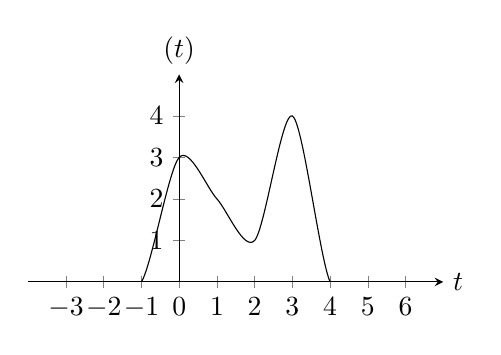
\begin{tikzpicture}
					\begin{axis} [width=195pt,height=120pt,
							axis x line=bottom,
							axis y line=middle,
							tick align=center,
							every axis x label/.style={at={(current axis.right of origin)},anchor=west},
							every axis y label/.style={at={(current axis.above origin)}, anchor=north east,above=0mm},
							xmin=-4, xmax=7,
							xtick={-3,...,6},
							xlabel=$t$,
							ymin=0, ymax=5,
							ytick={0,...,4},
							ylabel={$\img \left(t\right)$}]
						\addplot[smooth]
						coordinates {(-3,0) (-2,0) (-1,0) (0,3) (1,2) (2,1) (3,4) (4,0) (5,0) (6,0)};
					\end{axis}
				\end{tikzpicture}
				 & ~
				\text{(b)}
				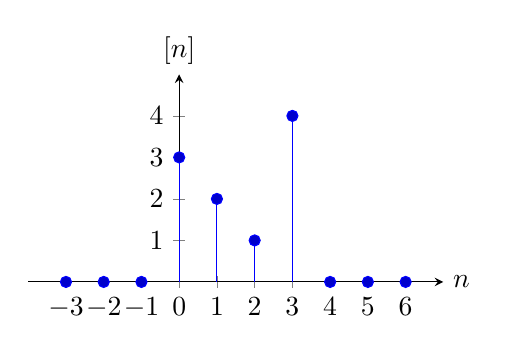
\begin{tikzpicture}
					\begin{axis} [width=195pt,height=120pt,
							axis x line=bottom,
							axis y line=middle,
							tick align=center,
							every axis x label/.style={at={(current axis.right of origin)},anchor=west},
							every axis y label/.style={at={(current axis.above origin)}, anchor=north east,above=0mm},
							xmin=-4, xmax=7,
							xtick={-3,...,6},
							xlabel=$n$,
							ymin=0, ymax=5,
							ytick={0,...,4},
							ylabel={$\img \left[n\right]$}]
						\addplot+[ycomb] plot coordinates {(-3,0) (-2,0) (-1,0) (0,3) (1,2) (2,1) (3,4) (4,0) (5,0) (6,0)};
					\end{axis}
				\end{tikzpicture}
			\end{array}
		$
	}
	\caption{(a) A continuous signal, and (b) a discrete signal obtained by sampling the continuous signal at the times $t=n$.}
	\label{fig:contdiscsignal}
\end{figure}

%\begin{dspPlot}[xlabel=n,ylabel={$f\left[n\right]$}]{-3, 6}{-1, 4.2}
%    \dspTapsAt[linecolor=blue!60]{-3}{0 0 0 3 2 1 4 0 0 0}
%\end{dspPlot}

%\psset{unit=.75cm}
%\begin{center}
%\begin{pspicture}(-4,-1)(6.5,6)
%    \psaxes[Dx=1,dx=1,Dy=1,dy=1,linewidth=0.75pt]{->}(0,0)(-3.95,0)(7,5)[$n$,-90][$f\left[n\right]$,180]
%    \dspTapsAt[linewidth=2pt,linecolor=blue!60]{-4}{0 0 0 0 3 2 1 4 0 0 0}
%    \psdot[linecolor=blue!60,dotsize=6pt,linewidth=2pt](-3,0) 
%    \psdot[linecolor=blue!60,dotsize=6pt,linewidth=2pt](-2,0) 
%    \psdot[linecolor=blue!60,dotsize=6pt,linewidth=2pt](-1,0) 
%    \psdot[linecolor=blue!60,dotsize=6pt,linewidth=2pt](0,3) 
%    \psdot[linecolor=blue!60,dotsize=6pt,linewidth=2pt](1,2) 
%    \psdot[linecolor=blue!60,dotsize=6pt,linewidth=2pt](2,1) 
%    \psdot[linecolor=blue!60,dotsize=6pt,linewidth=2pt](3,4) 
%    \psdot[linecolor=blue!60,dotsize=6pt,linewidth=2pt](4,0) 
%    \psdot[linecolor=blue!60,dotsize=6pt,linewidth=2pt](5,0) 
%    \psdot[linecolor=blue!60,dotsize=6pt,linewidth=2pt](6,0) 
%\end{pspicture}
%\end{center}

%
%\begin{figure}[h]
%\begin{center}
%\begin{tikzpicture}
%\begin{axis} [width=300pt,height=120pt,
%	axis x line=bottom, 
%	axis y line=middle, 
%	tick align=center,
%	every axis x label/.style={at={(current axis.right of origin)},anchor=west},
%	every axis y label/.style={at={(current axis.above origin)}, anchor=north east,above=0mm},
%	xmin=-4, xmax=7,
%	xtick={-3,...,6},
%	xlabel=$n$,
%	ymin=0, ymax=5,
%	ytick={0,...,4},
%	ylabel={$f\left[n\right]$}]
%\addplot+[ycomb] plot coordinates {(-3,0) (-2,0) (-1,0) (0,3) (1,2) (2,1) (3,4) (4,0) (5,0) (6,0)};
%\end{axis} 
%\end{tikzpicture}
%\end{center}
%\caption{A discrete signal.} 
%\label{fig:dicretesignal}
%\end{figure}



%\psset{unit=1cm}
%\begin{center}
%\begin{pspicture}(-3.5,-2)(6.5,2)
%   \psaxes[Dx=1,dx=1,Dy=1,dy=1]{->}(0,0)(-3.2,-1.25)(6.5,1.25)
%  \psplot[xunit=0.5cm,linecolor=red,linewidth=1.5pt,plotpoints = 100]{-\psPiTwo}{\psPiFour}{x RadToDeg sin}
%\end{pspicture}
%\end{center}

%
The signal in \fig{\ref{fig:contdiscsignal}}{b} is a function that takes on the values $\img \left[0\right] = 3$, $\img \left[1\right] = 2$, $\img \left[2\right] = 1$ and $\img \left[3\right] = 4$ and all other values are zero, $\img \left[n\right] = 0$. In most of the book we will work with discrete signals. In many cases it will be convenient to write discrete signals as vectors. Using vector notation we will write the previous signal, in the interval $n \in \left[0,6 \right],$ as a column vector $\boldimg = \left[3, 2, 1, 4, 0, 0, 0\right]^T$, where $T$ denotes transpose.
%

%Images and sequences are stored in a computer as arrays of numbers. 

\subsection{Images}

An image is a two dimensional array of values: $\boldimg \in \mathbb{R}^{M \times N}$, where $N$ is the image width and $M$ is the image height. A grayscale image is then just an array of numbers such as the following (in this example, intensity values are scaled between 0 and 256):


%Sequences are three dimensional and we will write them as $\img \left[n, m, t \right]$. 
%For a computer, an image of size $18\times18$ pixels will stored as 
% Can you guess the object that appears in this image?
%
%\begin{figure}
%\begin{center}
%\begin{tikzpicture} 
%\begin{axis}[ width=350pt,height=240pt,
%	mesh/ordering=y varies,
%	view={-20}{45},
%	xlabel={$n$}, ylabel={$m$}, zlabel={$\img \left[n, m \right]$}
%	]  
%%\addplot3[surf,mesh/cols=18,mesh/rows=18,colormap/blackwhite,domain=0:255,shader=flat] 
%\addplot3+[ycomb]
%coordinates { 
%%(0,0,160) (1,0,175) (2,0,171) (3,0,168) (4,0,168) (5,0,172) (6,0,164) (7,0,158) (8,0,167) (9,0,173) (10,0,167) (11,0,163) (12,0,162) (13,0,164) (14,0,160) (15,0,159) (16,0,163) (17,0,162) (0,1,149) (1,1,164) (2,1,172) (3,1,175) (4,1,178) (5,1,179) (6,1,176) (7,1,118) (8,1,97) (9,1,168) (10,1,175) (11,1,171) (12,1,169) (13,1,175) (14,1,176) (15,1,177) (16,1,165) (17,1,152) (0,2,161) (1,2,166) (2,2,182) (3,2,171) (4,2,170) (5,2,177) (6,2,175) (7,2,116) (8,2,109) (9,2,169) (10,2,177) (11,2,173) (12,2,168) (13,2,175) (14,2,175) (15,2,159) (16,2,153) (17,2,123) (0,3,171) (1,3,174) (2,3,177) (3,3,175) (4,3,167) (5,3,161) (6,3,157) (7,3,138) (8,3,103) (9,3,112) (10,3,157) (11,3,164) (12,3,159) (13,3,160) (14,3,165) (15,3,169) (16,3,148) (17,3,144) (0,4,163) (1,4,163) (2,4,162) (3,4,165) (4,4,167) (5,4,164) (6,4,178) (7,4,167) (8,4,77) (9,4,55) (10,4,134) (11,4,170) (12,4,167) (13,4,162) (14,4,164) (15,4,175) (16,4,168) (17,4,160) (0,5,173) (1,5,164) (2,5,158) (3,5,165) (4,5,180) (5,5,180) (6,5,150) (7,5,89) (8,5,61) (9,5,34) (10,5,137) (11,5,186) (12,5,186) (13,5,182) (14,5,175) (15,5,165) (16,5,160) (17,5,164) (0,6,152) (1,6,155) (2,6,146) (3,6,147) (4,6,169) (5,6,180) (6,6,163) (7,6,51) (8,6,24) (9,6,32) (10,6,119) (11,6,163) (12,6,175) (13,6,182) (14,6,181) (15,6,162) (16,6,148) (17,6,153) (0,7,134) (1,7,135) (2,7,147) (3,7,149) (4,7,150) (5,7,147) (6,7,148) (7,7,62) (8,7,36) (9,7,46) (10,7,114) (11,7,157) (12,7,163) (13,7,167) (14,7,169) (15,7,163) (16,7,146) (17,7,147) (0,8,135) (1,8,132) (2,8,131) (3,8,125) (4,8,115) (5,8,129) (6,8,132) (7,8,74) (8,8,54) (9,8,41) (10,8,104) (11,8,156) (12,8,152) (13,8,156) (14,8,164) (15,8,156) (16,8,141) (17,8,144) (0,9,151) (1,9,155) (2,9,151) (3,9,145) (4,9,144) (5,9,149) (6,9,143) (7,9,71) (8,9,31) (9,9,29) (10,9,129) (11,9,164) (12,9,157) (13,9,155) (14,9,159) (15,9,158) (16,9,156) (17,9,148) (0,10,172) (1,10,174) (2,10,178) (3,10,177) (4,10,177) (5,10,181) (6,10,174) (7,10,54) (8,10,21) (9,10,29) (10,10,136) (11,10,190) (12,10,180) (13,10,179) (14,10,176) (15,10,184) (16,10,187) (17,10,182) (0,11,177) (1,11,178) (2,11,176) (3,11,173) (4,11,174) (5,11,180) (6,11,150) (7,11,27) (8,11,101) (9,11,94) (10,11,74) (11,11,189) (12,11,188) (13,11,186) (14,11,183) (15,11,186) (16,11,188) (17,11,187) (0,12,160) (1,12,160) (2,12,163) (3,12,163) (4,12,161) (5,12,167) (6,12,100) (7,12,45) (8,12,169) (9,12,166) (10,12,59) (11,12,136) (12,12,184) (13,12,176) (14,12,175) (15,12,177) (16,12,185) (17,12,186) (0,13,147) (1,13,150) (2,13,153) (3,13,155) (4,13,160) (5,13,155) (6,13,56) (7,13,111) (8,13,182) (9,13,180) (10,13,104) (11,13,84) (12,13,168) (13,13,172) (14,13,171) (15,13,164) (16,13,168) (17,13,167) (0,14,184) (1,14,182) (2,14,178) (3,14,175) (4,14,179) (5,14,133) (6,14,86) (7,14,191) (8,14,201) (9,14,204) (10,14,191) (11,14,79) (12,14,172) (13,14,220) (14,14,217) (15,14,205) (16,14,209) (17,14,200) (0,15,184) (1,15,187) (2,15,192) (3,15,182) (4,15,124) (5,15,32) (6,15,109) (7,15,168) (8,15,171) (9,15,167) (10,15,163) (11,15,51) (12,15,105) (13,15,203) (14,15,209) (15,15,203) (16,15,210) (17,15,205) (0,16,191) (1,16,198) (2,16,203) (3,16,197) (4,16,175) (5,16,149) (6,16,169) (7,16,189) (8,16,190) (9,16,173) (10,16,160) (11,16,145) (12,16,156) (13,16,202) (14,16,199) (15,16,201) (16,16,205) (17,16,202) (0,17,153) (1,17,149) (2,17,153) (3,17,155) (4,17,173) (5,17,182) (6,17,179) (7,17,177) (8,17,182) (9,17,177) (10,17,182) (11,17,185) (12,17,179) (13,17,177) (14,17,167) (15,17,176) (16,17,182) (17,17,180)
%(0,17,160) (0,16,149) (0,15,161) (0,14,171) (0,13,163) (0,12,173) (0,11,152) (0,10,134) (0,9,135) (0,8,151) (0,7,172) (0,6,176) (0,5,160) (0,4,147) (0,3,184) (0,2,184) (0,1,191) (0,0,153) (1,17,175) (1,16,164) (1,15,166) (1,14,175) (1,13,163) (1,12,164) (1,11,155) (1,10,135) (1,9,132) (1,8,156) (1,7,173) (1,6,178) (1,5,160) (1,4,150) (1,3,182) (1,2,187) (1,1,198) (1,0,149) (2,17,170) (2,16,172) (2,15,182) (2,14,177) (2,13,162) (2,12,158) (2,11,146) (2,10,147) (2,9,131) (2,8,151) (2,7,178) (2,6,176) (2,5,162) (2,4,153) (2,3,178) (2,2,193) (2,1,203) (2,0,154) (3,17,168) (3,16,175) (3,15,171) (3,14,175) (3,13,165) (3,12,165) (3,11,147) (3,10,149) (3,9,125) (3,8,145) (3,7,177) (3,6,173) (3,5,162) (3,4,155) (3,3,175) (3,2,182) (3,1,197) (3,0,155) (4,17,168) (4,16,178) (4,15,170) (4,14,167) (4,13,167) (4,12,180) (4,11,169) (4,10,150) (4,9,115) (4,8,144) (4,7,178) (4,6,174) (4,5,161) (4,4,160) (4,3,179) (4,2,124) (4,1,175) (4,0,173) (5,17,172) (5,16,179) (5,15,177) (5,14,161) (5,13,164) (5,12,180) (5,11,180) (5,10,147) (5,9,129) (5,8,149) (5,7,181) (5,6,180) (5,5,167) (5,4,154) (5,3,133) (5,2,32) (5,1,150) (5,0,182) (6,17,164) (6,16,175) (6,15,175) (6,14,157) (6,13,178) (6,12,150) (6,11,163) (6,10,149) (6,9,132) (6,8,143) (6,7,175) (6,6,150) (6,5,100) (6,4,56) (6,3,87) (6,2,110) (6,1,169) (6,0,179) (7,17,158) (7,16,118) (7,15,116) (7,14,137) (7,13,167) (7,12,90) (7,11,50) (7,10,62) (7,9,74) (7,8,71) (7,7,53) (7,6,27) (7,5,45) (7,4,111) (7,3,191) (7,2,168) (7,1,189) (7,0,177) (8,17,167) (8,16,97) (8,15,109) (8,14,103) (8,13,77) (8,12,61) (8,11,24) (8,10,36) (8,9,54) (8,8,30) (8,7,20) (8,6,101) (8,5,169) (8,4,182) (8,3,200) (8,2,171) (8,1,190) (8,0,181) (9,17,173) (9,16,167) (9,15,169) (9,14,112) (9,13,55) (9,12,34) (9,11,32) (9,10,45) (9,9,41) (9,8,29) (9,7,29) (9,6,93) (9,5,166) (9,4,180) (9,3,204) (9,2,167) (9,1,173) (9,0,178) (10,17,167) (10,16,174) (10,15,177) (10,14,157) (10,13,135) (10,12,138) (10,11,119) (10,10,114) (10,9,104) (10,8,128) (10,7,135) (10,6,74) (10,5,59) (10,4,104) (10,3,191) (10,2,162) (10,1,160) (10,0,182) (11,17,162) (11,16,170) (11,15,174) (11,14,164) (11,13,170) (11,12,186) (11,11,163) (11,10,157) (11,9,156) (11,8,164) (11,7,190) (11,6,189) (11,5,137) (11,4,84) (11,3,79) (11,2,51) (11,1,145) (11,0,185) (12,17,162) (12,16,169) (12,15,169) (12,14,159) (12,13,167) (12,12,186) (12,11,175) (12,10,163) (12,9,152) (12,8,157) (12,7,180) (12,6,188) (12,5,184) (12,4,168) (12,3,171) (12,2,105) (12,1,156) (12,0,180) (13,17,164) (13,16,175) (13,15,175) (13,14,160) (13,13,162) (13,12,182) (13,11,181) (13,10,166) (13,9,156) (13,8,154) (13,7,179) (13,6,185) (13,5,176) (13,4,172) (13,3,220) (13,2,203) (13,1,202) (13,0,177) (14,17,160) (14,16,176) (14,15,176) (14,14,165) (14,13,163) (14,12,175) (14,11,181) (14,10,168) (14,9,164) (14,8,159) (14,7,177) (14,6,183) (14,5,175) (14,4,171) (14,3,216) (14,2,209) (14,1,199) (14,0,167) (15,17,159) (15,16,177) (15,15,159) (15,14,169) (15,13,175) (15,12,165) (15,11,162) (15,10,163) (15,9,156) (15,8,158) (15,7,184) (15,6,186) (15,5,177) (15,4,164) (15,3,205) (15,2,202) (15,1,201) (15,0,176) (16,17,162) (16,16,164) (16,15,153) (16,14,149) (16,13,168) (16,12,160) (16,11,148) (16,10,146) (16,9,141) (16,8,156) (16,7,187) (16,6,188) (16,5,185) (16,4,168) (16,3,208) (16,2,209) (16,1,205) (16,0,182) (17,17,162) (17,16,151) (17,15,122) (17,14,144) (17,13,160) (17,12,164) (17,11,153) (17,10,147) (17,9,144) (17,8,148) (17,7,182) (17,6,188) (17,5,186) (17,4,167) (17,3,200) (17,2,205) (17,1,202) (17,0,180)
%};
%\end{axis} 
%\end{tikzpicture}
%\end{center}
%\caption{A discrete 2D signal.} 
%\label{fig:disc2Dsignal_plot}
%\end{figure}
%
%
%Similarly to 1D signals, we can write this 2D signal as a matrix:
\[
	\begin{array}{cc}
		\boldimg = &
		%{\tiny
		\left[
			\begin{smallmatrix} 160 & 175 & 171 & 168 & 168 & 172 & 164 & 158 & 167 & 173 & 167 & 163 & 162 & 164 & 160 & 159 & 163 & 162\\ 149 & 164 & 172 & 175 & 178 & 179 & 176 & 118 & 97 & 168 & 175 & 171 & 169 & 175 & 176 & 177 & 165 & 152\\ 161 & 166 & 182 & 171 & 170 & 177 & 175 & 116 & 109 & 169 & 177 & 173 & 168 & 175 & 175 & 159 & 153 & 123\\ 171 & 174 & 177 & 175 & 167 & 161 & 157 & 138 & 103 & 112 & 157 & 164 & 159 & 160 & 165 & 169 & 148 & 144\\ 163 & 163 & 162 & 165 & 167 & 164 & 178 & 167 & 77 & 55 & 134 & 170 & 167 & 162 & 164 & 175 & 168 & 160\\ 173 & 164 & 158 & 165 & 180 & 180 & 150 & 89 & 61 & 34 & 137 & 186 & 186 & 182 & 175 & 165 & 160 & 164\\ 152 & 155 & 146 & 147 & 169 & 180 & 163 & 51 & 24 & 32 & 119 & 163 & 175 & 182 & 181 & 162 & 148 & 153\\ 134 & 135 & 147 & 149 & 150 & 147 & 148 & 62 & 36 & 46 & 114 & 157 & 163 & 167 & 169 & 163 & 146 & 147\\ 135 & 132 & 131 & 125 & 115 & 129 & 132 & 74 & 54 & 41 & 104 & 156 & 152 & 156 & 164 & 156 & 141 & 144\\ 151 & 155 & 151 & 145 & 144 & 149 & 143 & 71 & 31 & 29 & 129 & 164 & 157 & 155 & 159 & 158 & 156 & 148\\ 172 & 174 & 178 & 177 & 177 & 181 & 174 & 54 & 21 & 29 & 136 & 190 & 180 & 179 & 176 & 184 & 187 & 182\\ 177 & 178 & 176 & 173 & 174 & 180 & 150 & 27 & 101 & 94 & 74 & 189 & 188 & 186 & 183 & 186 & 188 & 187\\ 160 & 160 & 163 & 163 & 161 & 167 & 100 & 45 & 169 & 166 & 59 & 136 & 184 & 176 & 175 & 177 & 185 & 186\\ 147 & 150 & 153 & 155 & 160 & 155 & 56 & 111 & 182 & 180 & 104 & 84 & 168 & 172 & 171 & 164 & 168 & 167\\ 184 & 182 & 178 & 175 & 179 & 133 & 86 & 191 & 201 & 204 & 191 & 79 & 172 & 220 & 217 & 205 & 209 & 200\\ 184 & 187 & 192 & 182 & 124 & 32 & 109 & 168 & 171 & 167 & 163 & 51 & 105 & 203 & 209 & 203 & 210 & 205\\ 191 & 198 & 203 & 197 & 175 & 149 & 169 & 189 & 190 & 173 & 160 & 145 & 156 & 202 & 199 & 201 & 205 & 202\\ 153 & 149 & 153 & 155 & 173 & 182 & 179 & 177 & 182 & 177 & 182 & 185 & 179 & 177 & 167 & 176 & 182 & 180 \end{smallmatrix}\right]
		%}
	\end{array}
\]

This matrix represents an image of size $18 \times 18$ pixels as encoded in a computer. Can you guess what object appears in the array?
The goal of a computer vision system is to {\bf reorganize} this array of numbers into a meaningful representation of the scene depicted in the image. The next image shows the same array of values but visualized as gray levels.


% in figure \ref{fig:disc2Dsignal}. Again, it is hard to grasp the content of the image by just looking at this matrix. Figure \ref{fig:disc2Dsignal_image} visualizes the matrix as an image where each value is shown as a different gray-scale value. 


%It is also convenient to encode images as a 1D vector by concatenating all the image columns into a long column vector of $M \times N$ values. 

%\marginnote{}[-1.27cm]

\begin{figure}[h!]
	\centerline{
		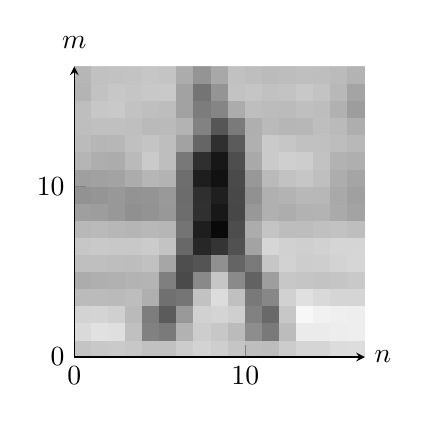
\begin{tikzpicture}\begin{axis}[width=150pt,height=150pt,
					mesh/ordering=y varies,
					view={0}{90},
					ymin=0, ymax=17,
					xmin=0, xmax=17,
					axis on top,
					axis x line=bottom,
					axis y line=left,
					tick align=inside,
					every axis x label/.style={at={(current axis.right of origin)},anchor=west},
					every axis y label/.style={at={(current axis.north west)}, anchor=north west,above=1mm},
					xlabel={$n$}, ylabel={$m$}, zlabel={$z$}
				]
				\addplot3[surf,mesh/cols=18,mesh/rows=18,colormap/blackwhite,domain=0:255,shader=flat]
				coordinates {
						%(0,0,160) (1,0,175) (2,0,171) (3,0,168) (4,0,168) (5,0,172) (6,0,164) (7,0,158) (8,0,167) (9,0,173) (10,0,167) (11,0,163) (12,0,162) (13,0,164) (14,0,160) (15,0,159) (16,0,163) (17,0,162) (0,1,149) (1,1,164) (2,1,172) (3,1,175) (4,1,178) (5,1,179) (6,1,176) (7,1,118) (8,1,97) (9,1,168) (10,1,175) (11,1,171) (12,1,169) (13,1,175) (14,1,176) (15,1,177) (16,1,165) (17,1,152) (0,2,161) (1,2,166) (2,2,182) (3,2,171) (4,2,170) (5,2,177) (6,2,175) (7,2,116) (8,2,109) (9,2,169) (10,2,177) (11,2,173) (12,2,168) (13,2,175) (14,2,175) (15,2,159) (16,2,153) (17,2,123) (0,3,171) (1,3,174) (2,3,177) (3,3,175) (4,3,167) (5,3,161) (6,3,157) (7,3,138) (8,3,103) (9,3,112) (10,3,157) (11,3,164) (12,3,159) (13,3,160) (14,3,165) (15,3,169) (16,3,148) (17,3,144) (0,4,163) (1,4,163) (2,4,162) (3,4,165) (4,4,167) (5,4,164) (6,4,178) (7,4,167) (8,4,77) (9,4,55) (10,4,134) (11,4,170) (12,4,167) (13,4,162) (14,4,164) (15,4,175) (16,4,168) (17,4,160) (0,5,173) (1,5,164) (2,5,158) (3,5,165) (4,5,180) (5,5,180) (6,5,150) (7,5,89) (8,5,61) (9,5,34) (10,5,137) (11,5,186) (12,5,186) (13,5,182) (14,5,175) (15,5,165) (16,5,160) (17,5,164) (0,6,152) (1,6,155) (2,6,146) (3,6,147) (4,6,169) (5,6,180) (6,6,163) (7,6,51) (8,6,24) (9,6,32) (10,6,119) (11,6,163) (12,6,175) (13,6,182) (14,6,181) (15,6,162) (16,6,148) (17,6,153) (0,7,134) (1,7,135) (2,7,147) (3,7,149) (4,7,150) (5,7,147) (6,7,148) (7,7,62) (8,7,36) (9,7,46) (10,7,114) (11,7,157) (12,7,163) (13,7,167) (14,7,169) (15,7,163) (16,7,146) (17,7,147) (0,8,135) (1,8,132) (2,8,131) (3,8,125) (4,8,115) (5,8,129) (6,8,132) (7,8,74) (8,8,54) (9,8,41) (10,8,104) (11,8,156) (12,8,152) (13,8,156) (14,8,164) (15,8,156) (16,8,141) (17,8,144) (0,9,151) (1,9,155) (2,9,151) (3,9,145) (4,9,144) (5,9,149) (6,9,143) (7,9,71) (8,9,31) (9,9,29) (10,9,129) (11,9,164) (12,9,157) (13,9,155) (14,9,159) (15,9,158) (16,9,156) (17,9,148) (0,10,172) (1,10,174) (2,10,178) (3,10,177) (4,10,177) (5,10,181) (6,10,174) (7,10,54) (8,10,21) (9,10,29) (10,10,136) (11,10,190) (12,10,180) (13,10,179) (14,10,176) (15,10,184) (16,10,187) (17,10,182) (0,11,177) (1,11,178) (2,11,176) (3,11,173) (4,11,174) (5,11,180) (6,11,150) (7,11,27) (8,11,101) (9,11,94) (10,11,74) (11,11,189) (12,11,188) (13,11,186) (14,11,183) (15,11,186) (16,11,188) (17,11,187) (0,12,160) (1,12,160) (2,12,163) (3,12,163) (4,12,161) (5,12,167) (6,12,100) (7,12,45) (8,12,169) (9,12,166) (10,12,59) (11,12,136) (12,12,184) (13,12,176) (14,12,175) (15,12,177) (16,12,185) (17,12,186) (0,13,147) (1,13,150) (2,13,153) (3,13,155) (4,13,160) (5,13,155) (6,13,56) (7,13,111) (8,13,182) (9,13,180) (10,13,104) (11,13,84) (12,13,168) (13,13,172) (14,13,171) (15,13,164) (16,13,168) (17,13,167) (0,14,184) (1,14,182) (2,14,178) (3,14,175) (4,14,179) (5,14,133) (6,14,86) (7,14,191) (8,14,201) (9,14,204) (10,14,191) (11,14,79) (12,14,172) (13,14,220) (14,14,217) (15,14,205) (16,14,209) (17,14,200) (0,15,184) (1,15,187) (2,15,192) (3,15,182) (4,15,124) (5,15,32) (6,15,109) (7,15,168) (8,15,171) (9,15,167) (10,15,163) (11,15,51) (12,15,105) (13,15,203) (14,15,209) (15,15,203) (16,15,210) (17,15,205) (0,16,191) (1,16,198) (2,16,203) (3,16,197) (4,16,175) (5,16,149) (6,16,169) (7,16,189) (8,16,190) (9,16,173) (10,16,160) (11,16,145) (12,16,156) (13,16,202) (14,16,199) (15,16,201) (16,16,205) (17,16,202) (0,17,153) (1,17,149) (2,17,153) (3,17,155) (4,17,173) (5,17,182) (6,17,179) (7,17,177) (8,17,182) (9,17,177) (10,17,182) (11,17,185) (12,17,179) (13,17,177) (14,17,167) (15,17,176) (16,17,182) (17,17,180)
						(0,17,160) (0,16,149) (0,15,161) (0,14,171) (0,13,163) (0,12,173) (0,11,152) (0,10,134) (0,9,135) (0,8,151) (0,7,172) (0,6,176) (0,5,160) (0,4,147) (0,3,184) (0,2,184) (0,1,191) (0,0,153) (1,17,175) (1,16,164) (1,15,166) (1,14,175) (1,13,163) (1,12,164) (1,11,155) (1,10,135) (1,9,132) (1,8,156) (1,7,173) (1,6,178) (1,5,160) (1,4,150) (1,3,182) (1,2,187) (1,1,198) (1,0,149) (2,17,170) (2,16,172) (2,15,182) (2,14,177) (2,13,162) (2,12,158) (2,11,146) (2,10,147) (2,9,131) (2,8,151) (2,7,178) (2,6,176) (2,5,162) (2,4,153) (2,3,178) (2,2,193) (2,1,203) (2,0,154) (3,17,168) (3,16,175) (3,15,171) (3,14,175) (3,13,165) (3,12,165) (3,11,147) (3,10,149) (3,9,125) (3,8,145) (3,7,177) (3,6,173) (3,5,162) (3,4,155) (3,3,175) (3,2,182) (3,1,197) (3,0,155) (4,17,168) (4,16,178) (4,15,170) (4,14,167) (4,13,167) (4,12,180) (4,11,169) (4,10,150) (4,9,115) (4,8,144) (4,7,178) (4,6,174) (4,5,161) (4,4,160) (4,3,179) (4,2,124) (4,1,175) (4,0,173) (5,17,172) (5,16,179) (5,15,177) (5,14,161) (5,13,164) (5,12,180) (5,11,180) (5,10,147) (5,9,129) (5,8,149) (5,7,181) (5,6,180) (5,5,167) (5,4,154) (5,3,133) (5,2,32) (5,1,150) (5,0,182) (6,17,164) (6,16,175) (6,15,175) (6,14,157) (6,13,178) (6,12,150) (6,11,163) (6,10,149) (6,9,132) (6,8,143) (6,7,175) (6,6,150) (6,5,100) (6,4,56) (6,3,87) (6,2,110) (6,1,169) (6,0,179) (7,17,158) (7,16,118) (7,15,116) (7,14,137) (7,13,167) (7,12,90) (7,11,50) (7,10,62) (7,9,74) (7,8,71) (7,7,53) (7,6,27) (7,5,45) (7,4,111) (7,3,191) (7,2,168) (7,1,189) (7,0,177) (8,17,167) (8,16,97) (8,15,109) (8,14,103) (8,13,77) (8,12,61) (8,11,24) (8,10,36) (8,9,54) (8,8,30) (8,7,20) (8,6,101) (8,5,169) (8,4,182) (8,3,200) (8,2,171) (8,1,190) (8,0,181) (9,17,173) (9,16,167) (9,15,169) (9,14,112) (9,13,55) (9,12,34) (9,11,32) (9,10,45) (9,9,41) (9,8,29) (9,7,29) (9,6,93) (9,5,166) (9,4,180) (9,3,204) (9,2,167) (9,1,173) (9,0,178) (10,17,167) (10,16,174) (10,15,177) (10,14,157) (10,13,135) (10,12,138) (10,11,119) (10,10,114) (10,9,104) (10,8,128) (10,7,135) (10,6,74) (10,5,59) (10,4,104) (10,3,191) (10,2,162) (10,1,160) (10,0,182) (11,17,162) (11,16,170) (11,15,174) (11,14,164) (11,13,170) (11,12,186) (11,11,163) (11,10,157) (11,9,156) (11,8,164) (11,7,190) (11,6,189) (11,5,137) (11,4,84) (11,3,79) (11,2,51) (11,1,145) (11,0,185) (12,17,162) (12,16,169) (12,15,169) (12,14,159) (12,13,167) (12,12,186) (12,11,175) (12,10,163) (12,9,152) (12,8,157) (12,7,180) (12,6,188) (12,5,184) (12,4,168) (12,3,171) (12,2,105) (12,1,156) (12,0,180) (13,17,164) (13,16,175) (13,15,175) (13,14,160) (13,13,162) (13,12,182) (13,11,181) (13,10,166) (13,9,156) (13,8,154) (13,7,179) (13,6,185) (13,5,176) (13,4,172) (13,3,220) (13,2,203) (13,1,202) (13,0,177) (14,17,160) (14,16,176) (14,15,176) (14,14,165) (14,13,163) (14,12,175) (14,11,181) (14,10,168) (14,9,164) (14,8,159) (14,7,177) (14,6,183) (14,5,175) (14,4,171) (14,3,216) (14,2,209) (14,1,199) (14,0,167) (15,17,159) (15,16,177) (15,15,159) (15,14,169) (15,13,175) (15,12,165) (15,11,162) (15,10,163) (15,9,156) (15,8,158) (15,7,184) (15,6,186) (15,5,177) (15,4,164) (15,3,205) (15,2,202) (15,1,201) (15,0,176) (16,17,162) (16,16,164) (16,15,153) (16,14,149) (16,13,168) (16,12,160) (16,11,148) (16,10,146) (16,9,141) (16,8,156) (16,7,187) (16,6,188) (16,5,185) (16,4,168) (16,3,208) (16,2,209) (16,1,205) (16,0,182) (17,17,162) (17,16,151) (17,15,122) (17,14,144) (17,13,160) (17,12,164) (17,11,153) (17,10,147) (17,9,144) (17,8,148) (17,7,182) (17,6,188) (17,5,186) (17,4,167) (17,3,200) (17,2,205) (17,1,202) (17,0,180)
					};
			\end{axis}
		\end{tikzpicture}
	}
	\caption{Grayscale image showing a person walking in the street. This tiny image has only $18\times18$ pixels.}
	%\label{fig:disc2Dsignal_image}
\end{figure}


When we want to make explicit the location of a pixel we will write $\img \left[n, m \right]$, where $n \in \left[0,N-1 \right]$ and $m \in \left[0,M-1 \right]$ are the indices for the horizontal and vertical dimensions, respectively. Each value in the array indicates the intensity of the image in that location. For color images we will have three channels, one for each color.

Although images are discrete signals, in some cases it is useful to work on the continuous domain as it simplifies the derivation of analytical solutions. This was the case in the previous chapter where we used the image gradient in the continuous domain and then approximated it in the discrete space domain. In those cases we will write images as $\img (x,y)$ and video sequences as $\img (x,y,t)$.


%\centerline{
%\begin{dspBlocks}{1}{4}
%$image~in$~~ & \BDfilter{System}  & ~~$image~out$
%  \ncline{->}{1,1}{1,2}
%  \ncline{->}{1,2}{1,3}
%\end{dspBlocks}
%}
%

\subsection{Properties of a Signal}

Here are some important quantities that are useful to characterize signals. As most signals represent physical quantities, a lot of the terminology used to describe them is borrowed from physics.

Both continuous and discrete signals can be classified according to its extend. {\bf Infinite length}
\index{Signals!Infinite length}
signals are signals that extend over the entire support $\img \left[n \right]$ for $n \in (-\infty, \infty)$. {\bf Finite length} \index{Signals!Finite length}
signals have non-zero values on a compact time interval and they are zero outside, i.e. $\img \left[n \right] = 0$ for $n \notin S$ where $S$ is a finite length interval.
A signal $\img \left[n \right]$ is {\bf periodic}
\index{Signals!Periodic}
if there is a value $N$ such that $\img \left[n \right] = \img \left[n + k N\right]$ for all $n$ and $k$. A periodic signal is an infinite length signal.


%%
%%
An important quantity is the mean value of a signal often called the {\bf DC value}.
\index{Signals!DC value}
\marginnote{DC means {\bf direct current} and it comes from electrical engineering. Although most signals have nothing to do with currents, the term DC is still commonly used.}[-.1in]
In the case of an image, the DC component is the average intensity of the image. For a finite signal of length $N$ (or a periodic signal), the {\bf DC value} is
\begin{equation}
	\mu = \frac{1}{N} \sum_{n=0}^{N-1} \img \left[n\right]
\end{equation}
If the signal is infinite, the average value is
\begin{equation}
	\mu = \lim_{N \xrightarrow{} \infty} \frac{1}{2N+1} \sum_{n=-N}^{N} \img \left[n\right]
\end{equation}


Another important quantity to characterize a signal is its energy. Following the same analogy with physics, the {\bf energy of a signal}
\index{Signals!Energy}
is defined as the sum of squared magnitude values:
\begin{equation}
	E = \sum_{n = -\infty}^{\infty} \left| \img  \left[n\right] \right| ^2
\end{equation}
\marginnote{Signal energy and energy of a physical quantity are equivalent up to a normalization constant. For instance, the energy dissipated by a resistance $R$ with voltage $v(t)$ is
	\begin{equation*}
		E = \frac{1}{R} \int_{-\infty}^{\infty} v(t) ^2 dt
	\end{equation*}
}[1in]

Signal are further classified as {\bf finite energy} and {\bf infinite energy} signals.
\index{Signals!Finite energy}
\index{Signals!Infinite energy}
Finite length signals are finite energy and periodic signals are infinite energy signals when measuring the energy in the whole time axis.

If we want to compare two signals, we can use the squared Euclidean distance (squared L2 norm) between them:
\begin{equation}
	D^2 = \frac{1}{N} \sum_{n=0}^{N-1} \left| \img_1 \left[n\right] - \img_2 \left[n\right] \right| ^2
\end{equation}
However, the euclidean distance (L2) is a poor metric when we are interested in comparing the content of the two images and the building better metrics is an important area of research. Sometimes, the metric is L2 but in a different representation space than pixel values. We will talk about this more later in the book.

The same definitions apply also to continuous signals, where all the equations are analogous by replacing the sums with integrals. For instance, in the case of the energy of a continuous signal, we can write $E = \int_{-\infty}^{\infty} \left| \img  \left( t \right) \right|^2 dt$, which assumes that the integral is finite. Most natural signals will have infinite energy.

\section{Systems}

The kind of systems that we will study here take a signal, $\boldimgin$, as input, perform some computation, $f$, and output another signal, $\boldimgout = f(\boldimgin)$.

\begin{figure}[h!]
	\centerline{
		\tikzstyle{int}=[draw, minimum size=3em]\tikzstyle{init} = [pin edge={to-,thin,black}]
		\begin{tikzpicture}[node distance=0cm,auto,>=latex']
			\node [int] (box1) {$f$};
			\node [left of=box1,node distance=1.5cm] (input) {$\boldimgin $};
			\node [right of=box1,node distance=2.0cm] (output) {$\boldimgout$};
			\node (c) [right of=box1,node distance=3cm, coordinate] {};
			\path[->] (input) edge node {} (box1);
			\path[->] (box1) edge node {} (output);
		\end{tikzpicture}
	}
	\caption{System processing one signal.}
	\label{fig:genericfilterH}
\end{figure}

This transformation is very general and it can do all sorts of complex things: it could detect edges in images, recognize objects, detect motion in sequences, or apply aesthetic transformations to a picture. The function $f$ could be specified as a mathematical operation or as an algorithm.
As a consequence, it is very difficult to find a simple way of characterizing what the function $f$ does. In the next section we will study a simple class of functions $f$ that allow for a simple analytical characterization: linear systems.



%\subsection{Signal space}
%
%As we have done already several times, it is very useful to think of signals and images as vectors. Let us define the two finite length column vectors $f$ and $g$ of length $N$. $f$ and $g$ can be the sequence of numbers of a 1D signal or the concatenation of all the columns (or rows) of a 2D image into a 1D column vector. Although we have only worked with real signals and images, later we will manipulate also signals and images made of complex numbers. 
%
%Then we can define:
%
%The scalar product between two (complex) signals is:
%\begin{equation}
%\left<f, g \right> = \sum_{n=0}^{N-1} f\left[n\right] g^*\left[n\right] = f^T g^*
%\end{equation}
%where $^*$ denotes complex conjugate. Two signals are orthogonal if $\left<f, g \right> = 0$.
%
%The scalar product also induces a norm. The squared L2 norm of a signal is:
%\begin{equation}
%E_f = \|f||^2 = \left<f, f \right> = \sum_{n=0}^{N-1} \left| f\left[n\right] \right| ^2 = f^T f^*
%\end{equation}
%some times this is referred to as the energy of the signal.
%
%If we want to compare two signals, we can use the squared L2 distance:
%\begin{equation}
%d^2_{f,g} = \|f-g||^2 = \sum_{n=0}^{N-1} \left| f\left[n\right] - g\left[n\right] \right| ^2 = E_f+E_g-2\left<f, g \right>
%\end{equation}
%
%The set of signals with finite L2 norm form a Hilbert space. We can also define basis, other metrics, ... 
%
%
%
%The same applies to continuous functions. 
%
%%\subsection{Properties of a signal}
%%
%%Signals and images are very high dimensional sequences of numbers. One of our goals is to find representations that extract from the signal some basic quantities that allow us making explicit signal properties that might allow us to understand its content. Here are some important quantities:
%%
%%
%%DC value is the mean signal value\footnote{DC means {\em direct current} and it comes from electric engineering. Although most signals have nothing to do with currents, the term DC is still commonly used.}:
%%\begin{equation}
%%DC = \sum_{n} f\left[n\right]
%%\end{equation}
%%
%%The energy of the signal is defined as the squared L2 norm of the signal:
%%\begin{equation}
%%E = \| f \|^2 = \sum_{n} | f\left[n\right] |^2
%%\end{equation}
%%
%%For finite energy signals, there are other quantities of interest:
%%
%%Center of mass of the signal measure the average position where the signal variations are located:
%%\begin{equation}
%%\mu = \frac{1}{E} \sum_{n} n~ | f\left[n\right] |^2
%%\end{equation}
%%
%%The variance in the spatial domain measures how compact is the signal:
%%\begin{equation}
%%\sigma^2 = \frac{1}{E} \sum_{n} (n-\mu)^2~| f\left[n\right] | ^2
%%\end{equation}
%%
%%
%%For an image, the mean is a 2D vector and the co-variance is a $2 \times 2$ matrix.
%%
%
\subsection{Linear Systems}

%Figure~\ref{fig:genericfilterH} we show what a general filter looks like. It takes as input a signal $g$ and outputs the signal $f$ such that 
%\begin{equation}
%f = H (g)
%\label{eq:general_nonlin_filter}
%\end{equation}
%where $H$ is an arbitrary function. 
%
%\begin{figure}[h]
%\begin{center}
%\tikzstyle{int}=[draw, minimum size=3em]
%\tikzstyle{init} = [pin edge={to-,thin,black}]
%\begin{tikzpicture}[node distance=0cm,auto,>=latex']
%  \node [int] (box1) {H
%%    	\begin{tikzpicture}
%%	\begin{axis} [width=80pt,height=80pt,
%%	axis x line=middle, 
%%	axis y line=middle, 
%%	tick align=center,
%%	every axis x label/.style={at={(current axis.right of origin)},anchor=west,right=-4mm},
%%	every axis y label/.style={at={(current axis.above origin)}, anchor=north east,above=-3.5mm},
%%	xmin=-1.8, xmax=3,
%%	xtick=\empty,
%%	xlabel=$n$,
%%	ymin=-1.8, ymax=2.8,
%%	ytick=\empty,
%%	ylabel={$h\left[n\right]$}]
%%	\addplot+[ycomb] plot coordinates {(0,2) (1,-1) (2,-1)};
%%	\end{axis} 
%%	\end{tikzpicture}
%    };
%   \node [left of=box1,node distance=1.5cm] (input) {$g $};
%   \node [right of=box1,node distance=1.5cm] (output) {$f$};
%    %\node (b) [left of=box1,node distance=3cm, coordinate] {};
%    \node (c) [right of=box1,node distance=3cm, coordinate] {};
%    %\path[->] (b) edge node {Image~in} (box1);
%    \path[->] (input) edge node {} (box1);
%    \path[->] (box1) edge node {} (output);
%\end{tikzpicture}
%\end{center}
%\caption{Notation to describe a general non-linear filter that takes as input a signal $g$ and outputs a signal $f$ so that $f=H(g)$.} 
%\label{fig:genericfilterH}
%\end{figure}
%

% They are nice because there are powerful tools to describe and implement them. On the other hand they represent a very small portion of all the possible filters one could implement. Despite this limitation we will show in the next chapter how some simple linear filters are capable of creating very interesting applications. 


%Among all possible systems, the simplest ones are 
{\bf Linear systems}
\index{Systems!Linear}
represent a very small portion of all the possible systems one could implement, but we will see that they are capable of creating very interesting image transformations. A function $f$ is linear is it satisfies the following two properties:

\begin{eqnarray}
	f\left( \boldimg_1+\boldimg_2 \right) &=& f(\boldimg_1)+ f(\boldimg_2) \\ \nonumber
	f(a\boldimg) &=& af(\boldimg) ~~\text{~for any scalar~} a
\end{eqnarray}

Although the previous properties might seem simple, it is easy to get confused on when an operation can be or not represented by a linear function. Let's first check your intuition about what operations are linear and which ones are not. Which ones of the image transformations shown in \fig{\ref{fig:transformationsquizz}} can be written as linear systems? \footnote{Answer: All of them!}


\begin{figure}[t]
	\centerline{
		\includegraphics[width=1\linewidth]{figures/linear_image_filtering/whichoneislinear.png}
	}
	\caption{Which one of these four image transformations (rotation by 30 degrees, scaling by 1/2, color to grayscale, and defocusing) can be written as linear functions?}
	\label{fig:transformationsquizz}
\end{figure}

To make things more concrete, lets assume the input is a 1D signal with length $N$ that we will write as $\imgin \left[n \right]$, and the output is another 1D signal with length $M$ that we will write as $\imgout \left[n \right]$. Most of the times we will work with input and output pairs with the same length $M=N$. A linear system, in its most general form, can be written as follows:
\begin{equation}
	\imgout \left[n \right] = \sum_{k=0}^{N-1} h \left[n,k\right] \imgin \left[k \right] ~~~ for ~~~ n \in \left[0, M-1 \right]
	\label{eq:general_lin_filter}
\end{equation}
where each output value $\imgout \left[n \right]$ is a linear combination of values of the input signal $\imgin \left[n \right]$ with weights $h \left[n,k\right]$. The value $h \left[n,k\right]$ is the weight applied to the input sample $\imgin \left[k \right]$ to compute the output sample $\imgout \left[n \right]$.
To help visualizing the operation performed by the linear filter it is useful to write it in matrix form:
\begin{equation*}
	\begin{bmatrix}
		\imgout\left[ 0 \right] \\
		\imgout\left[ 1 \right] \\
		\vdots                  \\
		\imgout\left[ n \right] \\
		\vdots                  \\
		\imgout\left[ M-1 \right]
	\end{bmatrix}
	=
	\begin{bmatrix}
		h\left[0,0\right] ~   & ~ h\left[0,1\right] ~   & ~ ... ~                 & ~ h\left[0,N-1\right]   \\
		h\left[1,0\right] ~   & ~ h\left[1,1\right] ~   & ~ ... ~                 & ~ h\left[1,N-1\right]   \\
		\vdots ~              & ~  \vdots ~             & ~  \vdots ~             & ~  \vdots               \\
		\vdots ~              & ~  \vdots ~             & ~  h \left[n,k\right] ~ & ~  \vdots               \\
		\vdots ~              & ~  \vdots ~             & ~  \vdots ~             & ~  \vdots               \\
		h\left[M-1,0\right] ~ & ~ h\left[M-1,1\right] ~ & ~ ... ~                 & ~ h\left[M-1,N-1\right]
	\end{bmatrix}
	~
	\begin{bmatrix}
		\imgin\left[0\right] \\
		\imgin\left[1\right] \\
		\vdots               \\
		\imgin\left[k\right] \\
		\vdots               \\
		\imgin\left[N-1\right]
	\end{bmatrix}
\end{equation*}
which we will write in short form as $\boldimgout =  \mathbf{H} \boldimgin$.
The matrix $\mathbf{H}$ has size $M \times N$.% where $N$ is the length of the input signal $x \left[n \right]$ and $M$ is the length of the output signal $y \left[n \right]$. 
We will use the matrix formulation many times in this book.

A linear function can also be drawn as a {\bf fully connected layer} in a neural network, with weights $\mathbf{W} = \mathbf{H}$, where the output unit $i$, $\imgout \left[i \right]$, is a linear combination of the input signal $\boldimgin$ with weights given by the row vectors of $\mathbf{H}$. Graphically it looks like this:

\begin{figure}[h!]
	\centerline{
		\includegraphics[width=.4\linewidth]{figures/linear_image_filtering/linear_filter.eps}
	}
	\caption{A linear function drawn as a {\bf fully connected layer} in a neural network.}
\end{figure}

In two dimensions the equations are analogous. Each pixel of the output
image, $\imgout \left[n,m\right]$, is computed as a linear combination of pixels of the input image, $\imgin \left[n, m\right]$:
\begin{equation}
	\imgout \left[n,m \right] = \sum_{k=0}^{M-1} \sum_{l=0}^{N-1} h \left[n,m,k,l \right] \imgin \left[k,l \right]
	\label{eq:lin}
\end{equation}
By writing the images as column vectors, concatenating all the image columns into a long vector, we can also write the previous equation using matrices and vectors: $\boldimgout =  \mathbf{H} \boldimgin$.

\subsection{Linear Translation Invariant Systems}



Linear systems are still too general for us. So let's consider an even smaller family of systems: {\bf linear translation invariant} (LTI) {\bf systems}.

%\marginnote{
\begin{figure}
	\centerline{
		\includegraphics[width=.25\linewidth]{figures/linear_image_filtering/space_of_functions.eps}
	}
	%}
\end{figure}

Translation invariant systems are motivated by the following observation: typically, we don't know where within the image we expect to find any
given item (\fig{\ref{fig:translationInvar}}), so we often want to process the image in a spatially invariant manner, the same processing algorithm at every pixel.


\begin{figure}
	\centerline{
		\includegraphics[width=1\linewidth]{figures/linear_image_filtering/fredo_birds1.jpg}
	}
	\caption{A fundamental property of images is translation
		invariance--the same image may appear at arbitrary spatial positions
		within the image. {\em Source}: Fredo Durand.}
	\label{fig:translationInvar}
\end{figure}

An example of a translation invariant system is a function that takes as input an image and computes at each location a local average value of the pixels around in a window of $5 \times 5$ pixels:
\begin{equation}
	\imgout \left[n,m \right] = \frac{1}{25} \sum_{k=-2}^{2} \sum_{l=-2}^{2} \imgin \left[n+k,m+l \right]
\end{equation}

%A simple example of a translation invariant system is a system that performs the following operation: 
%the output for sample $n$ is twice the value of the input at that same time minus the sum of the two previous time steps. This is:
%\begin{eqnarray}
%y\left[0\right] &=& 2 x\left[0\right] - x\left[-1\right] - x\left[-2\right] \nonumber \\
%y\left[1\right] &=& 2 x\left[1\right] - x\left[0\right] - g\left[-1\right] \nonumber \\
%y\left[2\right] &=& 2 x\left[2\right] - x\left[1\right] - x\left[0\right] \nonumber \\
%... \nonumber \\
%y\left[n\right] &=& 2 x\left[n\right] - x\left[n-1\right] - x\left[n-2\right] 
%\end{eqnarray}
%
A system is an LTI system if it is linear and when we translate the input signal by $n_0, m_0$, then output is also translated by $n_0, m_0$:
\begin{equation}
	\imgout \left[ n - n_0, m-m_0 \right] = f \left( \imgin \left[ n-n_0, m-m_0 \right] \right)
\end{equation}
for any $n_0,m_0$. This property is called {\bf equivariant}
\index{Systems!Equivariant}
with respect to translation. Translation invariance and linearity impose a strong constraint on the form of \eqn{\ref{eq:general_lin_filter}}.

%Translation invariance imposes a strong constraint on the form of equation~\ref{eq:general_lin_filter}. The weighting, $\mathbf{h}$, for the linear combination of the input image pixels, $\mathbf{x}$, is only a function of the spatial offset from the pixels of $\mathbf{x}$.  

In that case, the linear system becomes a {\bf convolution} of the image data with some {\bf convolution kernel}. This operation is very important and we devote the rest of this chapter to study its properties.


\section{Convolution}

The convolution, denoted $\circ$, between a signal $\imgin \left[n \right]$ and the {\bf convolutional kernel} $h\left[n \right]$ is defined as follows:
\begin{equation}
	%y \left[n\right] = h \left[n\right] \circ x \left[n\right] =  %\sum_{k=0}^{N-1} h \left[n-k \right] x \left[k \right]
	\imgout \left[n\right] = h \left[n\right] \circ \imgin \left[n\right] =  \sum_{k=-\infty}^{\infty} h \left[n-k \right] \imgin \left[k \right]
	\label{eq:1dconv}
\end{equation}
The convolution computes the output values as a linear weighted sum. The weight between the input sample $\imgin \left[k \right]$ and the output sample $\imgout \left[n\right]$ is a function $h\left[n, k \right]$ that depends only on their relative position $n-k$. Therefore, $h\left[n, k \right]=h\left[n-k \right]$. If the signal $\imgin \left[n \right]$ has a finite length, $N$, then the sum is only done in the interval $k \in \left[0,N-1\right]$.

The convolution is related to the {\bf correlation} operator. In the correlation, the weights are defined as $h\left[n, k \right]=h\left[k-n \right]$. The convolution and the correlation use the same kernel but mirrored around the origin.
The correlation is also translation invariant as we will discuss at the end of the chapter.

\marginnote{Most of the literature in neural networks calls convolution to the correlation operator. As the kernels are learned, the distinction is not important most of the time.}

One important property of the convolution is that it is commutative:
$h\left[n\right] \circ \img \left[n\right] = \img \left[n\right] \circ h\left[n\right]$.
This property is easy to prove by changing the variables, $k = n - k'$, so that:
\begin{equation}
	%y \left[n\right] = h \left[n\right] \circ x \left[n\right] =  %\sum_{k=0}^{N-1} h \left[n-k \right] x \left[k \right]
	h \left[n\right] \circ \imgin \left[n\right] =
	\sum_{k=-\infty}^{\infty} h \left[n-k \right] \imgin \left[k \right] = \sum_{k'=-\infty}^{\infty} h \left[k' \right] \imgin \left[n-k' \right]  =
	\imgin \left[n\right] \circ h \left[n\right]
\end{equation}

The convolution operation can be described in words as: first take the kernel $h\left[k\right]$ and mirror it $h\left[-k \right]$, then shift the mirrored kernel so that the origin is at location $n$, then multiply the input values around location $n$ by the mirrored kernel and sum the result. Store the result in the output vector $\imgout \left[n\right]$. For instance, if the convolutional kernel has three non-zero values: $h\left[-1 \right] =1$,  $h\left[0 \right] = 2$ and $h\left[1 \right] = 3$, then the output value at location $n$ is $\imgout \left[n\right] = 3 \imgin \left[n-1\right]+2 \imgin \left[n\right] + 1 \imgin \left[n+1\right]$.


%where $N$ is the length of the signal $x\left[n \right]$. This definition assumes that $x\left[n \right]$ is zero outside of the interval $n \in \left[0,N-1\right]$. 
For finite length signals, it helps to make explicit the structure of the convolution writing it in matrix form. For instance, if the convolutional kernel has only three non-zero values, then:
\begin{equation}
	\begin{bmatrix}
		\imgout \left[ 0 \right] \\
		\imgout \left[ 1 \right] \\
		\imgout \left[ 2 \right] \\
		\vdots                   \\
		\imgout \left[ N-1 \right]
	\end{bmatrix}
	=
	\begin{bmatrix}
		h\left[0\right] ~ & ~ h\left[-1\right] ~ & ~ 0 ~                & ~ ... ~   & ~ 0               \\
		h\left[1\right] ~ & ~ h\left[0\right] ~  & ~ h\left[-1\right] ~ & ~... ~    & ~ 0               \\
		0 ~               & ~ h\left[1\right] ~  & ~ h\left[0\right] ~  & ~... ~    & ~ 0               \\
		\vdots ~          & ~  \vdots ~          & ~  \vdots ~          & ~  \vdots                     \\
		0 ~               & ~ 0 ~                & ~ 0 ~                & ~... ~    & ~ h\left[0\right]
	\end{bmatrix}
	%\begin{bmatrix}
	% h\left[0\right] ~&~ h\left[-1\right] ~&~ h\left[-2\right] ~&~ ... ~&~ h\left[1-N\right] \\
	% h\left[1\right] ~&~ h\left[0\right] ~&~ h\left[-1\right] ~&~... ~&~ h\left[2-N\right] \\
	% h\left[2\right] ~&~ h\left[1\right] ~&~ h\left[0\right] ~&~... ~&~ h\left[3-N\right] \\
	% \vdots ~&~  \vdots ~&~  \vdots ~&~  \vdots \\
	% h\left[N-1\right] ~&~ h\left[N-2\right] ~&~ h\left[N-3\right] ~&~... ~&~ h\left[0\right] 
	%\end{bmatrix}
	~
	\begin{bmatrix}
		\imgin \left[0\right] \\
		\imgin \left[1\right] \\
		\imgin \left[2\right] \\
		\vdots                \\
		\imgin \left[N-1\right]
	\end{bmatrix}
\end{equation}

This operation is much easier to understand if we draw it as a {\bf convolutional layer} of a neural network as shown in \fig{\ref{fig:conv_filter2_nn}}.
%For instance, if only three values of $\mathbf{h}$ are non-zero:

\begin{figure}[h!]
	\centerline{
		\includegraphics[width=.5\linewidth]{figures/linear_image_filtering/conv_filter2.eps}
	}
	\caption{A convolution represented as a layer in a neural network. Each output unit $i$, $\imgout \left[i \right]$, is a linear combination of the input signal values around location $i$ always using the same set of weights given by $\mathbf{h}$.}
	\label{fig:conv_filter2_nn}
\end{figure}
%Each output unit $i$, $\imgout \left[i \right]$, is a linear combination of the input signal values around location $i$ always using the same set of weights given by $\mathbf{h}$. 


In two dimensions, the processing is analogous:
the input filter is flipped vertically and horizontally, then slid over the
image to record the inner product with the image everywhere.
Mathematically, this is:
\begin{equation}
	\imgout \left[n,m\right] = h \left[n,m\right] \circ \imgin \left[n,m\right] =  \sum_{k,l}h \left[n-k,m-l \right] \imgin \left[k,l \right]
	\label{eq:2dconv}
\end{equation}
The next figure shows the result of a 2D convolution between a $3 \times 3$ kernel with a $9 \times 9$ image. The particular kernel used in the figure averages in the
vertical direction and takes differences horizontally. The output
image reflects that processing, with horizontal differences
accentuated and vertical changes diminished. To compute one of the pixels in the output image, we start with an input image patch of $3 \times 3$ pixels, we flip the convolutional kernel upside-down and left-right, and then we multiply all the pixels in the image patch with the corresponding flipped kernel values and we sum the results.

\begin{figure}[h!]
	\centerline{
		\includegraphics[width=1\linewidth]{figures/linear_image_filtering/circle_conv_example.eps}
	}
	\caption{
		Illustration of a 2D convolution of an input image with a kernel of size $3 \times 3$.
		%The images are shown with both their pixel values and the corresponding image intensities. 
		For the pixels in the boundary we assumed that input image has zero values outside its boundary.
		%The convolution is performed by first rotating the kernel $h$ and then multiplying and summing the pixel and kernel values inside each $3x3$ input window to compute the corresponding output pixels. 
		The red and green boxes show the input pixels used to compute the corresponding output pixels.
	}
	\label{fig:circle_2dconv}
\end{figure}










%
%
%
%Let's start with the 1D case. As example of a translation invariant filter is a filter for which the output for the sample $n$ is twice the value of the input at that same time minus the sum of the two previous time steps. This is:
%\begin{eqnarray}
%f\left[0\right] &=& 2 g\left[0\right] - g\left[-1\right] - g\left[-2\right] \nonumber \\
%f\left[1\right] &=& 2 g\left[1\right] - g\left[0\right] - g\left[-1\right] \nonumber \\
%f\left[2\right] &=& 2 g\left[2\right] - g\left[1\right] - g\left[0\right] \nonumber \\
%... \nonumber \\
%f\left[n\right] &=& 2 g\left[n\right] - g\left[n-1\right] - g\left[n-2\right] 
%\end{eqnarray}
%
%A filter is linear translation invariant (LTI) if it is linear and when we translate the input signal by $m$ samples, the output is also translated by $m$ samples. This means that the behavior of the filter does not change depending on the location of the input. 
%%\begin{eqnarray}
%%g \left[n \right] = 
%%\end{eqnarray}
%
%Linear translation invariance imposes a strong constraint on the form of equation~\ref{eq:general_lin_filter}. The weighting, $h$, for the linear combination of the input image pixels, $g$, is only a function of the spatial offset from the pixels of $g$.
%For a 1D signal, a linear convolution, denoted $\circ$, of h and g is:
%\begin{equation}
%f\left[n\right] = h \circ g =  \sum_{k=0}^{N-1}h \left[n-k \right] g \left[k \right]
%\label{eq:1dconv}
%\end{equation}
%for the previous example $h = \left[2, -1, -1\right]$. $N$ is the length of the signal $g\left[n \right]$ and we assume it is zero outside of the interval $n \in \left[0,N-1\right]$.
%
%\begin{figure}[h]
%\begin{center}
%\tikzstyle{int}=[draw, minimum size=3em]
%\tikzstyle{init} = [pin edge={to-,thin,black}]
%\begin{tikzpicture}[node distance=0cm,auto,>=latex']
%   \node [int] (box1) {
%    	\begin{tikzpicture}
%	\begin{axis} [width=80pt,height=80pt,
%	axis x line=middle, 
%	axis y line=middle, 
%	tick align=center,
%	every axis x label/.style={at={(current axis.right of origin)},anchor=west,right=-4mm},
%	every axis y label/.style={at={(current axis.above origin)}, anchor=north east,above=-3.5mm},
%	xmin=-1.8, xmax=3,
%	xtick=\empty,
%	xlabel=$n$,
%	ymin=-1.8, ymax=2.8,
%	ytick=\empty,
%	ylabel={$h\left[n\right]$}]
%	\addplot+[ycomb] plot coordinates {(0,2) (1,-1) (2,-1)};
%	\end{axis} 
%	\end{tikzpicture}
%    };
%   \node [left of=box1,node distance=3cm] (input) {$g \left[n \right]$};
%   \node [right of=box1,node distance=3cm] (output) {$f \left[n \right]$};
%    %\node (b) [left of=box1,node distance=3cm, coordinate] {};
%    \node (c) [right of=box1,node distance=3cm, coordinate] {};
%    %\path[->] (b) edge node {Image~in} (box1);
%    \path[->] (input) edge node {} (box1);
%    \path[->] (box1) edge node {} (output);
%\end{tikzpicture}
%\end{center}
%\caption{Example of a linear translation invariant signal processing module. The function inside the box correspond to the convolution kernel.} 
%\label{fig:genericfilter}
%\end{figure}
%
%Most of the filters we will use will have what is called finite support. A filter has finite support if the filter kernel $h$ has non-zero values only at a finite number of locations. In the signal processing literature those filters are called finite impulse response filters (FIR). 
%
%In the 1D case, it helps to make explicit the structure of the matrix:
%\begin{equation}
%\begin{bmatrix}
%f\left[ 0 \right] \\
%f\left[ 1 \right] \\
%f\left[ 2 \right] \\
%\vdots \\
%f\left[ N-1 \right]
%\end{bmatrix}
% =
%\begin{bmatrix}
%  h\left[0\right] ~&~ h\left[-1\right] ~&~ h\left[-2\right] ~&~ ... ~&~ h\left[1-N\right] \\
%  h\left[1\right] ~&~ h\left[0\right] ~&~ h\left[-1\right] ~&~... ~&~ h\left[2-N\right] \\
%  h\left[2\right] ~&~ h\left[1\right] ~&~ h\left[0\right] ~&~... ~&~ h\left[3-N\right] \\
%  \vdots ~&~  \vdots ~&~  \vdots ~&~  \vdots \\
%  h\left[N-1\right] ~&~ h\left[N-2\right] ~&~ h\left[N-3\right] ~&~... ~&~ h\left[0\right] 
% \end{bmatrix}
%~
% \begin{bmatrix}
%  g\left[0\right] \\
%  g\left[1\right] \\
%  g\left[2\right] \\
%  \vdots \\
%  g\left[N-1\right]
% \end{bmatrix}
%\end{equation}
%
%Figure~\ref{fig:1dconv} 
%shows the convolution of a kernel, h,
%with a 1D signal, g.  h and g are shown in the top row.
%Subsequent rows show the implementation.
%$h\left[m-k\right]$ is just h, offset by $m$ pixels and reversed.  We multiply
%this term-by-term with g and sum those weighted values of g[m] to form
%the output signal, f[m].
%
%%\begin{figure}
%%\centerline{
%%\includegraphics[width=0.8\linewidth]{figures/intro_signals/1dconv.jpg}
%%} 
%%\caption{Illustration in 1-d of the steps in computing the convolution
%% of a kernel h with a signal g.  Shifted and offset versions of the
%% kernel h provide the weights to construct f[m] from a 
%% linear combination of the samples of g[m].
%%} 
%%\label{fig:1dconv}
%%\end{figure}
%
%
%\begin{figure}
%\centerline{
%\[
%\begin{array}{ccc}
%\begin{tikzpicture}
%	\begin{axis} [width=100,height=120pt,
%	axis x line=middle, 
%	axis y line=middle, 
%	tick align=center,
%	every axis x label/.style={at={(current axis.right of origin)},anchor=west,right=0mm},
%	every axis y label/.style={at={(current axis.above origin)}, anchor=north east,above=0mm},
%	xmin=-2.8, xmax=5,
%	xtick=\empty,
%	%xtick={-2,0, 1,2,3,4},
%	xlabel=$n$,
%	ymin=-2.2, ymax=4.6,
%	%ytick=\empty,
%	ytick={-1,0,1,2},
%	ylabel={$h\left[n\right]$}]
%	\addplot+[ycomb] plot coordinates {(-2,0) (-1,0) (0,2) (1,-1) (2,-1) (3,0) (4,0)};
%	\end{axis} 
%	\end{tikzpicture}
%&
%~\begin{tikzpicture}
%	\begin{axis} [width=150,height=120pt,
%	axis x line=middle, 
%	axis y line=middle, 
%	tick align=center,
%	every axis x label/.style={at={(current axis.right of origin)},anchor=west,right=0mm},
%	every axis y label/.style={at={(current axis.above origin)}, anchor=north east,above=0mm},
%	xmin=-3.8, xmax=9.0,
%	xtick=\empty,
%	%xtick={-2,0, 1,2,3,4},
%	xlabel=$k$,
%	ymin=-2.2, ymax=4.6,
%	%ytick=\empty,
%	ytick={-1,0,1,2},
%	ylabel={$g\left[k\right]$}]
%	\addplot+[ycomb] plot coordinates {(-3,0) (-2,0) (-1,0) (0,2) (1,2) (2,2) (3,2) (4,1) (5,1) (6,1) (7,0) (8,0)};
%	\end{axis} 
%\end{tikzpicture}
%&
%~~\begin{tikzpicture}
%	\begin{axis} [width=150,height=120pt,
%	axis x line=middle, 
%	axis y line=middle, 
%	tick align=center,
%	every axis x label/.style={at={(current axis.right of origin)},anchor=west,right=0mm},
%	every axis y label/.style={at={(current axis.above origin)}, anchor=north east,above=0mm},
%	xmin=-3.8, xmax=9.0,
%	xtick=\empty,
%	%xtick={-2,0, 1,2,3,4},
%	xlabel=$n$,
%	ymin=-2.2, ymax=4.6,
%	%ytick=\empty,
%	ytick={-1,0,1,2,3,4},
%	ylabel={$f\left[n\right]$}]
%        % 4     2     0     0    -2    -1     0    -2    -1
%	\addplot+[ycomb] plot coordinates {(-3,0) (-2,0) (-1,0) (0,4) (1,2) (2,0) (3,0) (4,-2) (5,-1) (6,0) (7,-2) (8,-1)};
%	\end{axis} 
%\end{tikzpicture}
%\\
%%f\left[0\right] = \sum_k h\left[-k\right]  g\left[k\right]
%&
%~~\begin{tikzpicture}
%	\begin{axis} [width=150,height=120pt,
%	axis x line=middle, 
%	axis y line=middle, 
%	tick align=center,
%	every axis x label/.style={at={(current axis.right of origin)},anchor=west,right=0mm},
%	every axis y label/.style={at={(current axis.above origin)}, anchor=north east,above=0mm},
%	xmin=-3.8, xmax=9.0,
%	xtick=\empty,
%	%xtick={-2,0, 1,2,3,4},
%	xlabel=$k$,
%	ymin=-1.8, ymax=4.6,
%	%ytick=\empty,
%	ytick={-1,0,1,2},
%	ylabel={$h\left[-k\right]$}]
%	\addplot+[ycomb] plot coordinates {(-3,0) (-2,-1) (-1,-1) (0,2) (1,0) (2,0) (3,0) (4,0) (5,0) (6,0) (7,0) (8,0)};
%	\end{axis} 
%\end{tikzpicture}
%&
%~~\begin{tikzpicture}
%	\begin{axis} [width=150,height=120pt,
%	axis x line=middle, 
%	axis y line=middle, 
%	tick align=center,
%	every axis x label/.style={at={(current axis.right of origin)},anchor=west,right=0mm},
%	every axis y label/.style={at={(current axis.above origin)}, anchor=north east,above=0mm},
%	xmin=-3.8, xmax=9.0,
%	xtick=\empty,
%	%xtick={-2,0, 1,2,3,4},
%	xlabel=$n$,
%	ymin=-2.2, ymax=4.6,
%	%ytick=\empty,
%	ytick={-1,0,1,2,3,4},
%	ylabel={$h\left[-k\right] g\left[k\right]$}]
%        % 4     2     0     0    -2    -1     0    -2    -1
%	\addplot+[ycomb] plot coordinates {(-3,0) (-2,0) (-1,0) (0,4) (1,0) (2,0) (3,0) (4,0) (5,0) (6,0) (7,0) (8,0)};
%	\end{axis} 
%\end{tikzpicture}
%\\
%%f\left[1\right] = \sum_k h\left[1-k\right]  g\left[k\right]
%&
%~~\begin{tikzpicture}
%	\begin{axis} [width=150,height=120pt,
%	axis x line=middle, 
%	axis y line=middle, 
%	tick align=center,
%	every axis x label/.style={at={(current axis.right of origin)},anchor=west,right=0mm},
%	every axis y label/.style={at={(current axis.above origin)}, anchor=north east,above=0mm},
%	xmin=-3.8, xmax=9.0,
%	xtick=\empty,
%	%xtick={-2,0, 1,2,3,4},
%	xlabel=$k$,
%	ymin=-1.8, ymax=4.6,
%	%ytick=\empty,
%	ytick={-1,0,1,2},
%	ylabel={$h\left[1-k\right]$}]
%	\addplot+[ycomb] plot coordinates {(-3,0) (-2,0) (-1,-1) (0,-1) (1,2) (2,0) (3,0) (4,0) (5,0) (6,0) (7,0) (8,0)};
%	\end{axis} 
%\end{tikzpicture}
%&
%~~\begin{tikzpicture}
%	\begin{axis} [width=150,height=120pt,
%	axis x line=middle, 
%	axis y line=middle, 
%	tick align=center,
%	every axis x label/.style={at={(current axis.right of origin)},anchor=west,right=0mm},
%	every axis y label/.style={at={(current axis.above origin)}, anchor=north east,above=0mm},
%	xmin=-3.8, xmax=9.0,
%	xtick=\empty,
%	%xtick={-2,0, 1,2,3,4},
%	xlabel=$n$,
%	ymin=-2.2, ymax=4.6,
%	%ytick=\empty,
%	ytick={-1,0,1,2,3,4},
%	ylabel={$h\left[1-k\right] g\left[k\right]$}]
%        % 4     2     0     0    -2    -1     0    -2    -1
%	\addplot+[ycomb] plot coordinates {(-3,0) (-2,0) (-1,0) (0,-2) (1,4) (2,0) (3,0) (4,0) (5,0) (6,0) (7,0) (8,0)};
%	\end{axis} 
%\end{tikzpicture}
%\\
%%\vdots
%&
%\vdots
%\\
%%f\left[8\right] = \sum_k h\left[8-k\right]  g\left[k\right]
%&
%~~\begin{tikzpicture}
%	\begin{axis} [width=150,height=120pt,
%	axis x line=middle, 
%	axis y line=middle, 
%	tick align=center,
%	every axis x label/.style={at={(current axis.right of origin)},anchor=west,right=0mm},
%	every axis y label/.style={at={(current axis.above origin)}, anchor=north east,above=0mm},
%	xmin=-3.8, xmax=9.0,
%	xtick=\empty,
%	%xtick={-2,0, 1,2,3,4},
%	xlabel=$k$,
%	ymin=-1.8, ymax=4.6,
%	%ytick=\empty,
%	ytick={-1,0,1,2},
%	ylabel={$h\left[8-k\right]$}]
%	\addplot+[ycomb] plot coordinates {(-3,0) (-2,0) (-1,0) (0,0) (1,0) (2,0) (3,0) (4,0) (5,0) (6,-1) (7,-1) (8,2)};
%	\end{axis} 
%\end{tikzpicture}
%&
%~~\begin{tikzpicture}
%	\begin{axis} [width=150,height=120pt,
%	axis x line=middle, 
%	axis y line=middle, 
%	tick align=center,
%	every axis x label/.style={at={(current axis.right of origin)},anchor=west,right=0mm},
%	every axis y label/.style={at={(current axis.above origin)}, anchor=north east,above=0mm},
%	xmin=-3.8, xmax=9.0,
%	xtick=\empty,
%	%xtick={-2,0, 1,2,3,4},
%	xlabel=$n$,
%	ymin=-2.2, ymax=4.6,
%	%ytick=\empty,
%	ytick={-1,0,1,2,3,4},
%	ylabel={$h\left[8-k\right] g\left[k\right]$}]
%        % 4     2     0     0    -2    -1     0    -2    -1
%	\addplot+[ycomb] plot coordinates {(-3,0) (-2,0) (-1,0) (0,0) (1,0) (2,0) (3,0) (4,0) (5,0) (6,-1) (7,0) (8,0)};
%	\end{axis} 
%\end{tikzpicture}
%\end{array}
%\\
%\]
%} 
%\caption{Illustration in 1-d of the steps in computing the convolution
% of a kernel h with a signal g.  Shifted and offset versions of the
% kernel h provide the weights to construct f[m] from a 
% linear combination of the samples of g[m].
%} 
%\label{fig:1dconv}
%\end{figure}
%
%%\subsubsection{Examples}
%

Let's revisit the four image transformation examples from \fig{\ref{fig:transformationsquizz}} and ask a new question. Which ones of the image transformations shown in \fig{\ref{fig:transformationsquizz}} can be written as a convolution?
\footnote{Only C and D from \fig{\ref{fig:transformationsquizz}} can be implemented by convolutions.}%[-.4in]

As shown in \fig{\ref{fig:transformationsquizz2}}{a}, in the defocusing transformation each output pixel at location $n,m$ is the local average of the input pixels in a local neighborhood around location $n,m$, and this operation is the same regardless of what pixel output we are computing. Therefore, it can be written as a convolution. The rotation transformation (for a fix rotation) is a linear operation but it is not translation invariant. As illustrated in \fig{\ref{fig:transformationsquizz2}}{b}, different output pixels require looking at input pixels in a way that is location specific. At the top left corner, one wants to grab a pixel from, say, five pixels up and to the right, and from the bottom right one needs to grab the pixel from about five pixels down and to the left. So this rotation operation can't be written as a spatially invariant operation.

\begin{figure}[h!]
	\centerline{
		\sublabelnp{(a)}{
			\includegraphics[width=.48\linewidth]{figures/linear_image_filtering/whyrotationisnotconvolution_a.png}
		}
		\sublabelnp{(b)}{
			\includegraphics[width=.48\linewidth]{figures/linear_image_filtering/whyrotationisnotconvolution_b.png}
		}
	}
	\caption{(a) Defocusing an image can be written as a convolution. (b) Rotation can't be written as a convolution.}
	\label{fig:transformationsquizz2}
\end{figure}





%Intensity scaling: $f\left[m,n\right] = a \times g\left[m,n\right]$, where $a$ is a constant, is a linear operation and can be written as a convolutional filter ($h\left[0,0\right]=a$).
%
%Intensity shift: $f\left[m,n\right] = g\left[m,n\right] + a$ where $a$ is a constant is not a linear operator.
%
%Image shift: linear and can be written as a convolutional filter.
%
%Image rotation: linear but can not be written as a convolutional filter.
%
%Image scaling: linear but can not be written as a convolutional filter.



\subsection{Properties of the Convolution}\label{sec:linear_image_filtering:properties_of_the_convolution}

The convolution is a linear operation that will be extensively used thorough the book and it is important to be familiar with some of its properties.

\begin{itemize}
	\item {\bf Commutative}. As we have already discussed before the convolution is commutative,
	      \begin{equation}
		      h\left[n\right] \circ \img \left[n\right] = \img \left[n\right] \circ h\left[n\right]
	      \end{equation}
	      which means that the order of convolutions is irrelevant. This is not true for the correlation.

	\item {\bf Associative}. Convolutions can be applied in any order:
	      \begin{equation}
		      \img_1 \left[n\right] \circ \img_2 \left[n\right] \circ \img_3 \left[n\right] = \img_1\left[n\right] \circ (\img_2\left[n\right] \circ \img_3\left[n\right]) = (\img_1\left[n\right] \circ \img_2\left[n\right]) \circ \img_3\left[n\right] \label{eqn:linear_image_filtering:conv_associative_property}
	      \end{equation}
	      In practice, for finite length signals, the associative property might be affected by how boundary conditions are implemented.

	\item {\bf Distributive} with respect to the sum:
	      \begin{equation}
		      \img_1\left[n\right] \circ (\img_2\left[n\right] + \img_3\left[n\right] ) = \img_1\left[n\right] \circ \img_2\left[n\right] +  \img_1 \left[n\right] \circ \img_3 \left[n\right]
	      \end{equation}


	\item {\bf Shift}. Another interesting property involves shifting the two convolved functions. Let's consider the convolution $\imgout \left[n\right] = h\left[n\right] \circ \imgin \left[n\right]$. If the input signal, $\imgin \left[n\right]$, is translated by a constant $n_0$, i.e. $\imgin \left[n - n_0\right]$, the result of the convolution with the same kernel, $h\left[n\right]$, is the same output as before but translated by the same constant $n_0$:
	      \begin{equation}
		      \imgout \left[n-n_0\right] =  h\left[n\right] \circ \imgin \left[n-n_0\right]
	      \end{equation}
	      Translating the kernel is equivalent:
	      \begin{equation}
		      \imgout \left[n-n_0\right] =  h\left[n\right] \circ \imgin \left[n-n_0\right]  = h\left[n-n_0\right] \circ \imgin \left[n\right]
	      \end{equation}
	      \marginnote{
		      %Example of shift. 
		      Given the signal:
		      \\
		      \centerline{
			      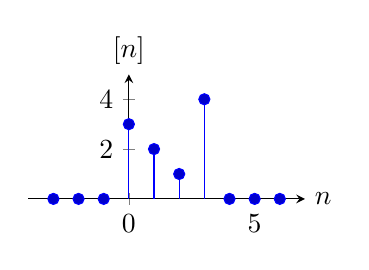
\begin{tikzpicture}
				      \begin{axis} [width=145pt,height=90pt,
						      axis x line=bottom,
						      axis y line=middle,
						      tick align=center,
						      every axis x label/.style={at={(current axis.right of origin)},anchor=west},
						      every axis y label/.style={at={(current axis.above origin)}, anchor=north east,above=0mm},
						      xmin=-4, xmax=7,
						      %xtick={-3,...,6},
						      xlabel=$n$,
						      ymin=0, ymax=5,
						      %ytick={0,...,4},
						      ylabel={$\img \left[n\right]$}]
					      \addplot+[ycomb] plot coordinates {(-3,0) (-2,0) (-1,0) (0,3) (1,2) (2,1) (3,4) (4,0) (5,0) (6,0)};
				      \end{axis}
			      \end{tikzpicture}}
		      \\
		      The signal $\img \left[n - n_0\right]$ is a shifted version of $\img \left[n\right]$. With $n_0 = 2$ this is \\
		      \centerline{
			      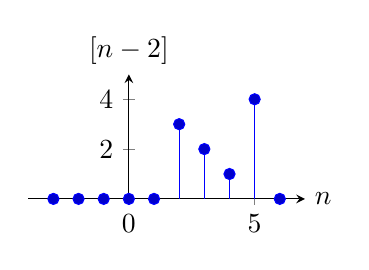
\begin{tikzpicture}
				      \begin{axis} [width=145pt,height=90pt,
						      axis x line=bottom,
						      axis y line=middle,
						      tick align=center,
						      every axis x label/.style={at={(current axis.right of origin)},anchor=west},
						      every axis y label/.style={at={(current axis.above origin)}, anchor=north east,above=0mm},
						      xmin=-4, xmax=7,
						      %xtick={-3,...,6},
						      xlabel=$n$,
						      ymin=0, ymax=5,
						      %ytick={0,...,4},
						      ylabel={$\img \left[n-2\right]$}]
					      \addplot+[ycomb] plot coordinates {
							      (-3,0) (-2,0) (-1,0) (0,0) (1,0) (2,3) (3,2) (4,1) (5,4) (6,0)
						      };
				      \end{axis}
			      \end{tikzpicture}
		      }
	      }[-1in]

	\item {\bf Support}. The convolution of a discrete signal of length $N$ with another discrete signal of length $M$ results in a discrete signal with length $L \leq M+N-1$.

	\item {\bf Identity}. The convolution also has an identity function, that is the {\bf impulse},
	      \index{Impulse}
	      $\delta \left[n\right]$, which takes the value 1 for $n=0$ and it is zero everywhere else:
	      \begin{equation}
		      \delta \left[n\right] =
		      \begin{cases}
			      1 & \quad \text{if } n=0      \\
			      0 & \quad \text{if } n \neq 0 \\
		      \end{cases}
	      \end{equation}
	      \marginnote{
		      The impulse function is:
		      \\[6pt]
		      \centerline{
			      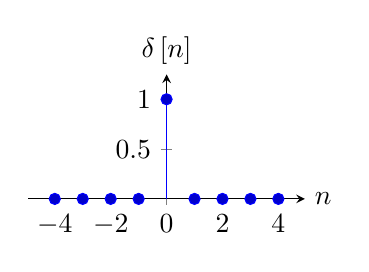
\begin{tikzpicture}\begin{axis} [width=145pt,height=90pt,
						      axis x line=bottom,
						      axis y line=middle,
						      tick align=center,
						      every axis x label/.style={at={(current axis.right of origin)},anchor=west},
						      every axis y label/.style={at={(current axis.above origin)}, anchor=north east,above=0mm},
						      xmin=-4.95, xmax=4.95,
						      %xtick={-3,...,6},
						      xlabel=$n$,
						      ymin=0, ymax=1.25,
						      ytick={0,0.5,1},
						      ylabel={$\delta \left[n\right]$}]
					      \addplot+[ycomb] plot coordinates {(-4,0) (-3,0) (-2,0) (-1,0) (0,1) (1,0) (2,0) (3,0) (4,0)};
				      \end{axis}
			      \end{tikzpicture}
		      }
	      }[-.6in]
	      The convolution of the impulse with any other signal, $\img \left[n\right]$, returns the same signal:
	      \begin{equation}
		      \delta \left[n\right] \circ \img \left[n\right] = \img \left[n\right]
	      \end{equation}
\end{itemize}

\subsection{Some Examples}

\Fig{\ref{fig:convExamps}} shows several simple convolution examples (each color channel is convolved with the same kernel). \Fig{\ref{fig:convExamps}}{a} shows a kernel with a single central non-zero element, $\delta \left[n,m\right]$, convolved with any image, gives back that same image.
% (even at the boundaries, by the way, since any pixels beyond the boundaries are multiplied by zero). 
\Fig{\ref{fig:convExamps}}{b} shows a kernel, $\delta \left[n,m-2\right]$, that produces a two pixel shift toward the right of the input image. The black line that appears on the left is due to the zero-boundary conditions (to be discussed in the next section) and it has a width of two pixels.  \Fig{\ref{fig:convExamps}}{c} shows the result of convolving the image with a kernel $0.5 \delta \left[n-2,m-2\right]+ 0.5 \delta \left[n+2,m+2\right]$. This results in two superimposed copies of the same image shifted diagonally in opposite directions. And finally, \fig{\ref{fig:convExamps}}{d} shows the result of convolving the image with a uniform kernel of all $1/25$.


\begin{figure}[t]
	\includegraphics[width=1\linewidth]{figures/linear_image_filtering/examples_cube2.eps}
	\caption{(a) An impulse convolved with the input image gives no
		change.  (b) A shifted impulse shifts the image.  (c) Sum of two shifted copies of the image.  (d) Image defocusing by computing a local average over windows of $5 \times 5$ pixels. All the examples use zero padding for handling boundary conditions.
	}
	\label{fig:convExamps}
\end{figure}

\subsection{Handling Boundaries}

When implementing a convolution, one is confronted with the question of what to do at the image boundaries.
There's really no satisfactory answer for how to handle the
boundaries that works well for all applications. One solution consists in omitting from the output any pixels that are affected by the input boundary. The issue with this is that the output will have a different size than the input and, for large convolutional kernels, there might be a large portion of the output image missing.
\marginnote{Only the green region contains values that can be computed, the rest will be affected by how we decide to handle the boundaries:
	\\[6pt]
	\centerline{
		\includegraphics[width=.4\linewidth]{figures/linear_image_filtering/regions_convolution.eps}
	}
}

The most general approach consists in extending the input image by adding additional pixels so that the output can have the same size as the input. So, for a kernel with support $\left[ -N, N \right] \times \left[-M, M\right]$, one has to add $N/2$ additional pixels left and right of the image and $M/2$ pixels at the top and bottom. Then, the output will have the same size as the original input image.

Some typical choices for how to pad the input image are (see \fig{\ref{fig:boundaries}}):
\begin{itemize}
	\item Zero padding: Set the pixels outside the boundary to zero (or to some other constant such as the mean image value). This is the default option in most neural networks.
	\item Circular padding: Extend the image by replicating the pixels from the other side. If the image has size $P \times Q$, circular padding consists of the following:
	      \begin{equation}
		      \imgin \left[n,m\right] = \imgin \left[(n)_P,(m)_Q\right]
	      \end{equation}
	      where $(n)_P$ denotes the modulo operation and $(n)_P$ is the reminder of $n/P$.

	      This padding transform the finite length signal into a periodic infinite length signal. Although this will introduce many artifacts, it is a convenient extension for analytical derivations.
	\item Mirror padding: Reflect the valid image pixels over the boundary of valid output pixels. This is the most common approach and the one that gives the best results.
	\item Repeat padding: Set the value to that of the nearest output image pixel with valid mask inputs.
\end{itemize}

\Fig{\ref{fig:boundaries}} shows different examples of boundary extensions. Boundary extensions are different ways of approximating the ground truth image that exists beyond the image boundary.
The top row shows how the image is extended beyond its boundary when using different types of boundary extensions (only the central part corresponds to the input). The middle row shows the output of the convolution (cropped to match the size of the input image). We can see that the zero-padding makes a darkening appear on the boundary of the image. This is not very desirable in general. The other padding methods seem to produce better visual results.


\begin{figure}
	\includegraphics[width=1\linewidth]{figures/linear_image_filtering/boundary.eps}
	\caption{Each row shows: (a) Different types of boundary extension. The last image shows the ground truth. (b) The output of convolving the image with a uniform kernel of size $11 \times 11$ with all the values equal to $1/121$. The output only shows the central region that corresponds to the input image without boundary extension. (c) The difference between each output and the ground truth output; see last column of (b). Note that the ground truth will not be available in practice.
	}
	\label{fig:boundaries}
\end{figure}

But which one is the best boundary extension? Ideally, we would to get a result that is a close as possible to the output we would get if we had access to a larger image. In this case we know what the larger image looks like as shown in the last column of \fig{\ref{fig:boundaries}}. For each boundary extension method, the final row shows the absolute value of the difference between the convolution output and the result obtained with the ground truth.

For the example of \fig{\ref{fig:boundaries}}, the error seems to be smaller when extending the image using mirror padding. On the other extreme, zero padding seems to be the worst.
%




%\section{Correlation and template matching}

%FIGURE: example letter detection, or face detection. Could be where is Waldo as well!

\subsection{Circular Convolution}

When convolving a finite length signal with a kernel, we have seen that it can be convenient to extend the signal beyond its boundary to reduce boundary artifacts. This trick is also very useful analytically and conduces to a special case of the convolution: the {\bf circular convolution} uses circular padding. The circular convolution of two signals, $h$ and $\imgin$, of length $N$ is defined as follows:

\begin{equation}
	\imgout \left[n\right] = h \left[n\right] \circ_N \imgin \left[n\right] =  \sum_{k=0}^{N-1} h \left[(n-k)_N \right] \imgin \left[k \right]
\end{equation}



In this formulation, the signal $h \left[ (n)_N \right]$ is the infinite periodic extension, with period $N$, of the finite length signal $h \left[n \right]$. The output of the circular convolution is a periodic signal with period $N$, $\imgout \left[n \right] = \imgout \left[(n)_N \right]$.


The circular convolution has the same properties than the convolution (e.g., is commutative.)

\marginnote{
	Writing the circular convolution in matrix form will look like:
	\\[6pt]
	\centerline{
		\includegraphics[width=.3\linewidth]{figures/linear_image_filtering/circ_conv.eps}
	}}[-.2in]

\subsection{Convolution in the Continuous Domain}
%
%Although in practice all the convolutions will be done in the discrete domain, the continuous domain is important for analytical derivations and for characterizing signals before they are captured by the camera. 
%
The convolution in the continuous domain is defined in the same way as with discrete signals but replacing the sums by integrals. Given two continuous signals $h(t)$ and $\imgin(t)$, the convolution operator is defined as follows:
\begin{equation}
	\imgout(t) = h(t) \circ \imgin (t) = \int_{-\infty}^{\infty} h(t-\tau) \imgin (\tau) d\tau
\end{equation}

The properties of the continuous domain convolution are analogous to the properties of the discrete convolution, with the commutative, associative and distributive relationships still holding.

We can also define the impulse, $\delta (t)$, in the continuous domain such that $\img(t) \circ \delta(t) = \img(t)$. The impulse is defined as being zero everywhere but at the origin where it takes an infinitely high value so that its integral is equal to 1:
\begin{equation}
	\int_{-\infty}^{\infty} \delta(t) dt = 1
\end{equation}
The impulse function is also called the impulse distribution (as it is not a function in the strict sense) or the Dirac delta function.
\marginnote{
	The delta distribution is usually represented with an arrow of height 1, indicating that it has an finite value at that point, and a finite area equal to 1:
	\\[6pt]
	\centerline{
		\begin{tikzpicture}
			\begin{axis} [width=120pt,height=100pt,
					axis x line=middle,
					axis y line=middle,
					tick align=center,
					every axis x label/.style={at={(current axis.right of origin)},anchor=west},
					every axis y label/.style={at={(current axis.above origin)}, anchor=north east,above=0mm},
					xmin=-.5, xmax=5,
					xtick={3},
					xticklabel={$a$},
					xlabel=$t$,
					ymin=-.5, ymax=2,
					ytick={0,1},
					ylabel={$\delta (t-a)$}]
				\addplot+[ycomb,mark=triangle] plot coordinates {(3,1)};
			\end{axis}
		\end{tikzpicture}
	}
}[-.1in]
The impulse has several important properties:
\begin{itemize}
	\item Scaling property: $\delta (at) =  \delta (t) / |a|$
	\item Symmetry: $\delta (-t) = \delta (t)$
	\item Sampling property: $\img (t) \delta (t-a) = \img(a) \delta (t-a)$ where $a$ is a constant. From this, we have the following:
	      \begin{equation}
		      \int_{-\infty}^{\infty} \img (t) \delta (t-a) dt = \img(a)
	      \end{equation}
	\item As in the discrete case, the continuous impulse is also the identity for the convolution: $\img(t) \circ \delta (t) = \img(t)$.
\end{itemize}

The impulse will be useful in analytical derivations and we will see it again in \chap{\ref{chapter:sampling}} when we discuss sampling.

\section{Cross-Correlation Versus Convolution}

Another form of writing a translation invariant filter is using the cross-correlation operator. The cross-correlation provides a simple technique to locate a template in an image.
The cross-correlation and the convolution are closely related.


The {\bf cross-correlation} operator (denoted by $\star$) between the image $\imgin$ and the kernel $h$ is written as follows:
\begin{equation}
	\imgout \left[n,m\right] = \imgin \star h =  \sum_{k,l=-N}^N \imgin \left[n+k,m+l \right] h \left[k,l \right]
\end{equation}
where the sum is done over the support of the filter $h$, which we assume is a square $(-N,N)\times(-N,N)$.
In the convolution, the kernel is inverted left-right and up-down, while in the cross-correlation is not. Remember that the convolution between image $\imgin$ and kernel $h$ is written as follows:
\begin{equation}
	\imgout \left[n,m\right] = \imgin \circ h = \sum_{k,l=-N}^N \imgin \left[n-k,m-l \right] h \left[k,l \right]
\end{equation}



\Fig{\ref{fig:corrvsconv}} illustrates the difference between the correlation and the convolution. In these examples, the kernel $h[n,m]$ is a triangle pointing up (the center of the triangle is $n=0$ and $m=0$) as shown in \fig{\ref{fig:corrvsconv}}{a}. When the input image is black (all zeros) with only four bright pixels, \fig{\ref{fig:corrvsconv}}{b}, this is the convolution of the triangle with four impulses, which results in four triangles pointing up (\fig{\ref{fig:corrvsconv}}[c]). However, the cross-correlation looks different; it still results in four copies of the triangles centered on each point, but the triangles are pointing downward (\fig{\ref{fig:corrvsconv}}[d]).

For the input image containing triangles pointing up and down, \fig{\ref{fig:corrvsconv}}{e}, the convolution will have its maximum output on the triangles points down, \fig{\ref{fig:corrvsconv}}{f}, while the correlation will output the maximum values in the center of the triangles pointing up (\fig{\ref{fig:corrvsconv}}[g]).


\begin{figure}[t]
	\centerline{
		\includegraphics[width=1\linewidth]{figures/linear_image_filtering/correlation_vs_convolution.eps}
	}
	\caption{Cross-correlation versus convolution. (a) Kernel. (b) and (e) are two input images. (c) and (f) are the output convolution with the kernel (a). (d) and (g) are the cross-correlation output with the kernel (a).}
	\label{fig:corrvsconv}
\end{figure}


Another important difference between the two operators is that the convolution is commutative and associative while the correlation is not. The correlation breaks the symmetry between the two functions $h$ and $\imgin$. For instance, in the correlation, shifting $h$ is not equivalent to shifting $\imgin$ (the output will move in opposite directions). Note that the cross-correlation and convolution outputs are identical when the kernel $h$ has central symmetry.



\subsection{Template Matching and Normalized Correlation}

% TODO: Switching f and h would be helpful in the previous sections as well. 
% I guess f suits better for the filter and h is commonly used as feature map (output after any hidden layer in NNs)



The goal of template matching is to find a small image patch within a larger image.
%For instance, \fig{\ref{fig:normcorr}} illustrates the detection of the ``a" letters through matching an example ``a''  template in a given text image, as shown in \fig{\ref{fig:normcorr}}{b}.
\Fig{\ref{fig:normcorr}} shows how to use template matching to detect all the occurrences of the letter ``a'' with an image of text, shown in \fig{\ref{fig:normcorr}}{b}. \Fig{\ref{fig:normcorr}}{a} shows the template of the letter ``a''.



\begin{figure}[t]
	\includegraphics[width=1\linewidth]{figures/linear_image_filtering/normcorr.eps}
	\caption{(a) Template. (b) Input image. (c) Correlation between input (b) and template (a). (d) Normalized correlation. e) Locations with cross-correlation above 75 percent of its maximum value.
	}
	\label{fig:normcorr}
\end{figure}

% correlation or cross-correlation ??

Cross-correlation is a potential method for template matching, but it has certain flaws. Consider matching the ``a'' template in \fig{\ref{fig:normcorr}}{a} in a given input image. Just by increasing the brightness of the image in different parts we can increase the filter response since correlation is essentially a multiplication between the kernel $h$ and any input image patch $p$  (note that all the values are positive in $p$ and $h$). In bright image regions we will have the maximum correlation values regardless of regions' content as shown in \fig{\ref{fig:normcorr}}{c}.

The normalized cross-correlation, at location $(n,m)$, is the dot product between a template, $h$, (normalized to be zero mean and unit norm) and the local image patch, $p$, centered at that location and with the same size as the kernel, normalized to be unit norm. This can be implemented with the following steps: First, we normalize the kernel $h$. The normalized kernel $\hat h$ is the result of making the kernel $h$ zero mean and unit norm. Then, the normalized cross-correlation is as follows (\fig{\ref{fig:normcorr}}{d}):
%\begin{equation}
%y\left[n,m\right] = \sum_{k,l=-N}^N 
%                \frac{
%                (x \left[n+k,m+l \right] - \mu_x \left[n,m \right])}
%                {\sigma_x \left[n,m \right]}
%                \frac{
%                (h \left[k,l \right] - \mu_h )}
%                {\sigma_h} 
%\end{equation}
%where 
%\begin{equation}
%\mu_h = \frac{1}{(2N+1)^2} \sum_{k,l=-N}^N h \left[k,l \right]
%\end{equation} 
%and 
%\begin{equation}
%\sigma^2_h = \frac{1}{(2N+1)^2} \sum_{k,l=-N}^N (h \left[k,l \right] - \mu_h)^2
%\end{equation} 
\begin{equation}
	\imgout \left[n,m\right]
	=
	\frac{1}{\sigma \left[n,m \right]}
	\sum_{k,l=-N}^N
	\imgin \left[n+k,m+l \right]
	\hat{h} \left[k,l \right]
\end{equation}
Note that this equation is similar to the correlation function, but the output is scaled by the local standard deviation, $\sigma \left[m,n \right]$, of the image patch centered in $(n,m)$ and with support $(-N,N)\times(-N,N)$, where $(-N,N)\times(-N,N)$ is the size of the kernel $h$. To compute the local standard deviation, we first compute the local mean, $\mu \left[n,m \right]$, as follows:
\begin{equation}
	\mu \left[n,m \right] = \frac{1}{(2N+1)^2} \sum_{k,l=-N}^N \imgin \left[n+k,m+l \right]
\end{equation}
And then we compute:
\begin{equation}
	\sigma^2 \left[n,m \right] = \frac{1}{(2N+1)^2} \sum_{k,l=-N}^N \left( \imgin \left[n+k,m+l \right] - \mu \left[n,m \right] \right) ^2
\end{equation}

\Fig{\ref{fig:normcorr}}{e} shows the detected copies of the template \fig{\ref{fig:normcorr}}{a} in the image \fig{\ref{fig:normcorr}}{b}. The red bounding boxes in \fig{\ref{fig:normcorr}}{e} correspond to the location with local maximum values of the normalized cross-correlation (\fig{\ref{fig:normcorr}}{d}) that are above a threshold chosen by hand.

%\begin{equation}
%{f}' = f - m_f \quad \text{where}  \quad m_f = \frac{1}{MN} %\sum_{n=0}^{N-1}\sum_{m=0}^{M-1} f \left[n,m \right] \label{zero-mean-signals}
%\end{equation}
%To further improve the robustness we can normalize both the filter $f$ and the applied image patch $g$ with standard deviations, eventually obtaining normalized cross-correlation (NCC) as:
%\begin{eqnarray}
%NCC(f,g) = \left< \bar{f}, \bar{g} \right> \quad  \text{where}  \quad  \bar{f} = \frac{f - m_f}{\sqrt{\left<f - m_f,f - m_f\right>}} =  \frac{f'}{\sqrt{\left<f,f'\right>}}, \nonumber \\
%								       \bar{g} = \frac{g - m_g}{\sqrt{\left<g - m_g,g - m_g\right>}} =  \frac{g'}{\sqrt{\left<f',f'\right>}}
%\end{eqnarray}
%Note that both $\bar{f}$ and $\bar{g}$ are unit norm vectors. Therefore $NCC(f,g)=\left< \bar{f}, \bar{g} \right> = ||\bar{f}|| \, ||\bar{g}|| \, cos \alpha = cos \alpha$ where $\alpha$ is the angle
%between the vectors $f'$ and $g'$.

%Another common method of comparing patches is through sum of squared distances (SSD), also referred to as squared L2 distance:
%\begin{equation}
%SSD(f,g) = || f- g ||^2 = \sum_n |f\left[n\right] - g\left[n\right]|^2 = E_f + E_g - 2\left<f,g\right>
%\end{equation}
%However this method also suffers in extreme illumination changes as the distance is strongly effected by the energy of the signals $E_f$ and $E_g$. 
%We can remove such undesired effects through L2 normalization of signals $\hat{f} = \frac{f}{||f||}$ and $\hat{g} = \frac{g}{||g||}$, and eventually obtain 
%normalized squared L2 distance:
%\begin{equation}
%SSD(\hat{f} ,\hat{g}) = ||\hat{f} - \hat{g} ||^2= E_{\hat{f}} + E_{\hat{g}} - 2\left<f,g\right> = 2 - 2\left<\hat{f} ,\hat{g} \right>
%\end{equation}
%where $E_{\hat{f}} = E_{\hat{g}} =1$ as $\hat{f}$ and $\hat{g}$ are unit norm vectors due to the normalization. An important factor to note here is that the distance is no longer effected by the norm of the signals, but it is merely defined 
%by the angle between two signals as follows:
%\begin{equation}
%SSD(\hat{f} ,\hat{g}) = 2 - 2 cos \theta \quad \text{since} \quad \left<\hat{f} ,\hat{g} \right> = ||\hat{f}|| \, ||\hat{g}|| \, cos \theta = cos \theta
%\end{equation}
%where $\theta$ is the angle between the vectors $f$ and $g$. The quantity $\left<\hat{f} ,\hat{g} \right>$ is also referred to as cosine similarity, a well known similarity metric that is essentially the cosine of the 
%angle between two vectors defined as follows:
%\begin{equation}
%cos_{sim}(f,g) = \frac{\left<f ,g\right>}{||f|| \, ||g||}
%\end{equation}
%Note that cosine similarity is bounded by the interval $\left[-1,+1\right]$ as $cos \theta$ is. Hence $SSD(\hat{f} ,\hat{g})$  is bounded by the interval $\left[0,4\right]$.

%If we want to have a measure of similarity between two signals that is invariant to overall image brightness, then a more appropriate measure is the angle.
%Note that both $NCC$ and $cos_{sim}$ are angular similarity measures and they are not effected by the energy of the signals such as illumination changes in images.
%The major difference between them is that $\theta$ in  $cos_{sim}$ is the angle between original signals $f$ and $g$ whereas  $\alpha$ in $NCC$ is the angle between the 
%zero-mean vectors  $f'$ and $g'$  defined in (\ref{zero-mean-signals}).

%Convolution and correlation operators are the main building blocks of the convolutional neural networks. 

% Maybe we can explain distance vs. similarity with the example SSD(squared l2) vs cos_sim. 

% Keypoints from Antonio:
%   + Talk about computing distances between signals.
%   + Talk about matched filters.
%   + Normalize correlation: measuring the angle.

%% older text
%\begin{equation}
%d^2(f,g) = <f,f> + <g,g> - 2<f,g>
%\end{equation}
%If we want to have a measure of similarity between two signals that is invariant to overall image brightness, then a more appropriate measure is the angle:

%\begin{equation}
%\frac{<f-m_f,g-m_g>}{\sqrt {<f-m_f,f-m_f>} \sqrt{<g-m_g,g-m_g>} }
%\end{equation}
%\begin{equation}
%m_f = \frac{1}{MN} \sum_{n=0}^{N-1}\sum_{m=0}^{M-1} f \left[n,m \right]
%\end{equation}

In the example of \fig{\ref{fig:normcorr}}, all the instances of the letter 'a' have been correctly detected. But this method is very fragile when used to detect objects and is useful only under very limited conditions. Normalized correlation will detect the object independently of location, but it will not be robust to any other changes such as rotation, scaling, and changes in appearance. Just changing the font of the letters will certainly make the approach fail.

\section{System Identification}

One important task that we will study is that of explaining the behavior of complex systems such as neural networks. For an LTI filter with kernel $h\left[n\right]$, the output from an impulse is $y\left[n\right] = h\left[n\right]$. The output of a translated impulse $\delta \left[n -n_0 \right]$ is $h \left[n -n_0 \right]$. This is why the kernel that defines an LTI system, $h\left[n\right]$, is also called the impulse response of the system.


\begin{figure}[h!]
	\centerline{
	\tikzstyle{int}=[draw, minimum size=3em]
	\tikzstyle{init} = [pin edge={to-,thin,black}]
	\begin{tikzpicture}[node distance=0cm,auto,>=latex']
		\node [int] (box1) {$h \left[ n \right]$};
		\node [left of=box1,node distance=1.5cm] (input) {$\delta \left[ n \right] $};
		\node [right of=box1,node distance=1.5cm] (output) {$h \left[ n \right]$};
		\node (c) [right of=box1,node distance=2.0cm, coordinate] {};
		\path[->] (input) edge node {} (box1);
		\path[->] (box1) edge node {} (output);
	\end{tikzpicture}
	}
	\caption{LTI system with impulse response $h\left[n\right]$.}
	\label{fig:genericfilterH}
\end{figure}

For an unknown system, one way of finding the convolution kernel $h$ consists in computing the output of the system when the input is an impulse.



Let's start with a beautiful example from  acoustics \cite{TraerE7856}. When you are in a room you often hear that sounds are distorted with echos (\fig{\ref{fig:impulse_response_room_a}}). The number and strength of the echos depend on the geometry of the room, whether it is full or empty and the materials in the walls and ceilings.

\begin{figure}
	\centerline{
		\includegraphics[width=.6\linewidth]{figures/linear_image_filtering/impulse_response_room_a1.eps}
	}
	\caption{As shown in the sketch, sounds produced by one speaking person reach a listener via multiple paths. What the person hears is the superposition of all those signals. Figure modified from \cite{TraerE7856}.}
	\label{fig:impulse_response_room_a}
\end{figure}


Interestingly the relationship between the sounds that are originated in one location and what a listener hears in another position are related by an LTI system. If you are in a room and you clap (which is a good approximation to an impulse of sound), the echoes that you hear are very close to the impulse response of the system formed by the acoustics of the room. Any sounds that originates at the location of your clap will produce a sound in the room that will be qualitatively similar to the convolution of the acoustic signal with the echoes that you hear before when you clapped. \Fig{\ref{fig:impulse_response_room_a2}} shows a recording made in a restaurant in Cambridge, Massachusetts.


\begin{figure}
	\centerline{
		\includegraphics[width=1\linewidth]{figures/linear_image_filtering/impulse_response_room_a2.eps}
	}
	\caption{(a) Apparatus used to measure the impulse response generated by a battery-powered speaker and a
		portable digital recorder. (b) Recorded acoustic impulse response of a room. Figure modified from \cite{TraerE7856}.}
	\label{fig:impulse_response_room_a2}
\end{figure}




% Figure from: Traer, J., McDermott, J.H. (2016) Statistics of natural reverberation enable perceptual separation of sound and space. Proceedings of the National Academy of Sciences, 113, E7856-E7865


\Fig{\ref{fig:impulse_response_room_b}}, adapted from \cite{TraerE7856}, shows a sketch of how a voice signal gets distorted by the impulse response of a room before it reaches the listener. The impulse response, $h (t)$, is modeled here as a sequence of four impulses, the first impulse corresponds to the direct path and the remaining three to the different paths inside the room, modeled with different delays ($T_i$) and amplitudes ($0 < a_i < 1$):
\begin{equation}
	h (t) = a_0 \delta (t)
	+ a_1 \delta \left(t-T_1 \right)
	+ a_2 \delta \left( t-T_2 \right)
	+ a_3 \delta \left( t-T_3 \right)
\end{equation}
The sound that reaches the listener is the superposition of four copies of the sound emitted by the speaker. This can be written as the convolution of the input sound, $\imgin (t)$, with room impulse response, $h (t)$:
\begin{equation}
	\imgout (t) = \imgin (t) \circ h(t) = a_0 \imgout (t)
	+ a_1 \imgin (t-T_1)
	+ a_2 \imgin (t-T_2)
	+ a_3 \imgin (t-T_3)
\end{equation}
which is shown graphically in \fig{\ref{fig:impulse_response_room_b}}.
\begin{figure}
	\centerline{
		\includegraphics[width=1\linewidth]{figures/linear_image_filtering/impulse_response_room_b.eps}
	}
	% Figure from: Traer, J., McDermott, J.H. (2016) Statistics of natural reverberation enable perceptual separation of sound and space. Proceedings of the National Academy of Sciences, 113, E7856-E7865
	\caption{Modified from \cite{TraerE7856}.}
	\label{fig:impulse_response_room_b}
\end{figure}

\section{Concluding Remarks}

A good foundation in signal processing is a valuable background for computer vision scientists and engineers. This short introduction should now allow you go deeper by consulting other specialized books.

But we are not done yet. In the next chapter we will study the Fourier transform, which will provide a useful characterization of signals and images.

%\reviewcomment{To be written.}


%
%\section{Special signals}
%
%There are two families of signals that deserve special attention due to their role in modeling linear systems: the impulse and sinusoidal waves.
%
%\subsection{The impulse}
%\label{section:impulse}
%
%One important discrete signal is the impulse (also called the Kronecker delta function). The impulse in 1D is the signal defined as:
%\begin{equation}
%\delta \left[n\right] =
%  \begin{cases}
%    1       & \quad \text{if } n=0\\
%    0       & \quad \text{if } n \neq 0 \\
%  \end{cases}
%\end{equation}
%it takes the value 1 for $n=0$ and it is zero everywhere else. 
%
%\begin{figure}[h]
%\begin{center}
%\begin{tikzpicture}
%\begin{axis} [width=200pt,height=80pt,
%	axis x line=bottom, 
%	axis y line=middle, 
%	tick align=center,
%	every axis x label/.style={at={(current axis.right of origin)},anchor=west},
%	every axis y label/.style={at={(current axis.above origin)}, anchor=north east,above=0mm},
%	xmin=-4, xmax=4,
%	xtick={-3,...,3},
%	xlabel=$n$,
%	ymin=0, ymax=1.4,
%	ytick={0,...,1},
%	ylabel={$\delta \left[n\right]$}]
%\addplot+[ycomb] plot coordinates {(-3,0) (-2,0) (-1,0) (0,1) (1,0) (2,0) (3,0)};
%\end{axis} 
%\end{tikzpicture}
%\end{center}
%\caption{Impulse signal.} 
%\label{fig:dicretesignal}
%\end{figure}
%
%This signal is important because it has some very useful properties. The most important one is that it behaves as the identity function for the convolution. The result of convolving a signal $g\left[n\right]$ with the impulse signal is the same signal:
%\begin{equation}
%f\left[n\right] = \delta \circ g =  \sum_{k}\delta \left[n-k \right] g \left[k \right] = g \left[n \right]
%\end{equation}
%Convolving a signal $f$ with a translated impulse $\delta \left[n -n_0 \right]$ results in a translated signal:
%\begin{equation}
%f\left[n -n_0 \right] = \delta \left[n -n_0 \right] \circ f \left[n \right] 
%\end{equation}
%
%For an LTI filter with kernel $h\left[n\right]$, the output from an impulse is $f\left[n\right] = h\left[n\right]$. The output of a translated impulse $\delta \left[n -n_0 \right]$ is $h \left[n -n_0 \right]$. This is why the filter kernel $h\left[n\right]$ is also called the impulse response of the system. For an unknown system, one way of finding the convolution kernel $h$ consists in computing the output of the system when the input is an impulse. 
%
%If you are in a room and you clap (which is a good approximation to an impulse of sound), the echoes that you hear are very close to the impulse response of the system formed by the acoustics of the room. Any sounds that originates at the location of your clap will produce a sound in the room that will be qualitatively similar to the convolution of the acoustic signal with the echoes that you hear before when you clapped. 
%
%To see how the shift operation works, let's see what happens in 1D. The linear system that shifts the signal by one sample can be written as $h\left[n\right] = \delta \left[n-1\right]$. In matrix form this is:
%\begin{equation}
%\begin{bmatrix}
%  0 ~&~ 0 ~&~ 0 ~&~ ... ~&~ 0~&~ 0 \\
%  1 ~&~ 0 ~&~ 0 ~&~... ~&~ 0~&~ 0 \\
%  0 ~&~ 1 ~&~ 0 ~&~... ~&~ 0 ~&~ 0\\
%  \vdots ~&~  \vdots ~&~  \vdots ~&~  \vdots \\
%  0~&~ 0 ~&~ 0 ~&~ ... ~&~ 1 ~&~ 0
% \end{bmatrix}
%~
% \begin{bmatrix}
%  g\left[0\right] \\
%  g\left[1\right] \\
%  g\left[2\right] \\
%  \vdots \\
%  g\left[N-1\right]
% \end{bmatrix}
% =
%  \begin{bmatrix}
%  0\\
%  g\left[0\right] \\
%  g\left[1\right] \\
%  \vdots \\
%  g\left[N-2\right]
% \end{bmatrix}
%\end{equation}
%The first zero is a boundary artifact (in this example we are using zero-padding to extend the signal). The rest of the signal is translated by 1 location.
%
%The set of impulse signals, $\delta \left[n-k \right]$, delayed for all values $k \in \left[0, N-1\right]$, constitutes a basis for the set of discrete signals defined in the domain $\left[0, N-1\right]$. Any discrete signal can be written as a linear combination of delayed impulse responses:
%\begin{equation}
%f\left[n \right] = \sum_{k=0}^{N-1} f\left[k \right] \delta \left[n - k\right]
%\end{equation}
%where the values $f\left[k \right]$ are the coefficients used for the linear combination of the set of impulses.
%
%In 2D, the impulse is
%\begin{equation}
%\delta \left[n,m\right] =
%  \begin{cases}
%    1       & \quad \text{if } n=0,~m=0\\
%    0       & \quad \text{either } n \neq 0 ~\text{or}~ m \neq 0\\
%  \end{cases}
%\end{equation}
%
%The 2D impulse is a separable function, meaning that it can be written as the product of two 1D functions, both impulses:
%\begin{equation}
%\delta \left[n,m\right] = \delta \left[n\right] \delta \left[m\right]
%\end{equation}
%Convolution by an impulse can be used to translate an image:
%\begin{equation}
%f\left[n -n_0,m-m_0 \right] = \delta \left[n -n_0, m-m_0 \right] \circ f \left[n,m \right] 
%\end{equation}
%Although this might seem like an obscure way of doing such a simple image operation, it is very useful for analytical derivations. 
%%\subsubsection{Rectangle}
%%
%%A comment on integral images. 
%%
%%\begin{equation}
%%\delta \left[n\right] =
%%  \begin{cases}
%%    1       & \quad \text{if } n=0\\
%%    0       & \quad \text{if } n \neq 0 \\
%%  \end{cases}
%%\end{equation}
%%it takes the value 1 for $n=0$ and it is zero everywhere else. 
%%
%%
%%\begin{figure}[h]
%%\begin{center}
%%\begin{tikzpicture}
%%\begin{axis} [width=200pt,height=80pt,
%%	axis x line=bottom, 
%%	axis y line=middle, 
%%	tick align=center,
%%	every axis x label/.style={at={(current axis.right of origin)},anchor=west},
%%	every axis y label/.style={at={(current axis.above origin)}, anchor=north east,above=0mm},
%%	xmin=-4, xmax=4,
%%	xtick={-3,...,3},
%%	xlabel=$n$,
%%	ymin=0, ymax=1.4,
%%	ytick={0,...,1},
%%	ylabel={$r \left[n\right]$}]
%%\addplot+[ycomb] plot coordinates {(-3,0) (-2,0) (-1,1) (0,1) (1,1) (2,0) (3,0)};
%%\end{axis} 
%%\end{tikzpicture}
%%\end{center}
%%\caption{Impulse signal.} 
%%\label{fig:dicretesignal}
%%\end{figure}
%
%The impulse can also be defined on the continuous domain. The continuous impulse is represented as $\delta (t)$ with $t \in \Re$. The impulse function is defined as being zero everywhere but at the origin where it takes an infinitely high value so that its integral is equal to 1:
%\begin{equation}
%\int_{-\infty}^{\infty} \delta(t) dt = 1
%\end{equation}
%The impulse function is also called the impulse distribution (as it is not a function in the strict sense) or the Dirac delta function. 
%
%The impulse has several important properties:
%\begin{itemize}
%\item Scaling property: $\delta (at) =  \delta (t) / |a|$
%\item Symmetry: $\delta (-t) = \delta (t)$
%\item Sampling property: $f(t) \delta (t-a) = f(a) \delta (t-a)$ where $a$ is a constant. From this, we have: 
%\begin{equation}
%\int_{-\infty}^{\infty} f(t) \delta (t-a) dt = f(a)
%\end{equation}
%\item As in the discrete case, the continuous impulse is also the identity for the convolution: $f(t) \circ \delta (t) = f(t)$.
%\end{itemize}
%
%This function will be useful in analytical derivations and we will see it come back in section \ref{section:sampling} when we discuss sampling.
%
